\documentclass[final, twoadvisors]{nddiss2e}
              % draft + 10pt/11pt/12pt + twoadvisors + textrefs review +
              % noinfo + twoadvisors + textrefs final + noinfo +
              % twoadvisors + textrefs

\usepackage{anyfontsize}
\usepackage{color}
\usepackage{enumitem}  % for indenting enumerated lists
\usepackage{gensymb}
\usepackage{listings}
\usepackage{siunitx}

\definecolor{deepblue}{rgb}{0,0,0.5}
\definecolor{deepred}{rgb}{0.6,0,0}
\definecolor{deepgreen}{rgb}{0,0.5,0}

\newcommand{\nuc}[2]{${}^{#1}\textrm{#2}$}
\newcommand{\mnuc}[2]{{}^{#1}\textrm{#2}}
\newcommand{\react}[4]{$#1(#2,#3)#4$}
\newcommand{\mreact}[4]{#1(#2,#3)#4}
\newcommand{\alpa}{\react{\mnuc{27}{Al}}{\textrm{p}}{\alpha}{\mnuc{24}{Mg}}}
\newcommand{\nag}{\react{\mnuc{14}{N}}{\alpha}{\gamma}{\mnuc{18}{F}}}
\newcommand{\squared}{${}^{2}$}

\newcommand\pythonstyle{\lstset{
    language=Python,
    basicstyle=\ttm,
    otherkeywords={self},             % Add keywords here
    keywordstyle=\ttb\color{deepblue},
    emph={MyClass,__init__},          % Custom highlighting
    emphstyle=\ttb\color{deepred},    % Custom highlighting style
    stringstyle=\color{deepgreen},
    frame=tb,                         % Any extra options here
    showstringspaces=false            %
}}
\lstnewenvironment{python}[1][]{\pythonstyle\lstset{#1}}{}

\begin{document}

% Everything before first chapter goes here
\frontmatter

\title{VERIFICATION OF RECOIL SEPARATOR PROPERTIES THROUGH DIRECT
       REACTION MEASUREMENTS}
\author{Michael Thaddeus Moran}
\work{Dissertation}
\degaward{Doctor of Philosophy}
\advisor{Mano\"{e}l Couder}
\secondadvisor{Michael C.\ F.\ Wiescher}
\department{Physics}

\maketitle

\begin{abstract}

The St.\ George recoil separator is designed to measure
$(\alpha,\gamma)$ cross sections of astrophysical interest in inverse
kinematics. The design of the separator allows for a relatively large
energy ($\pm7.5$\,\%~$\Delta E/E$) and angular ($\pm40$~mrad) acceptance
that must be verified across a wide range of electric and magnetic
rigidities before primary experimental work can begin. Additionally, the
beam rejection properties of the separator system must be determined to
ensure that the direct incident beam is adequately rejected such that
the produced recoils can be confidently measured. The commissioning work
to experimentally verify these properties, and the procedures used, will
be discussed.

Utilization of the separator for measuring cross sections of
astrophysical interest outside of the design parameters is an additional
benefit of the commissioning work and expands the potential domain of
study for the separator. The first such experiment to measure two strong
resonances in the \alpa{} cross section has been completed. This
reaction study is additionally a test of the separator's energy and
angular acceptances \emph{in situ} as a precursor to studying
$(\alpha,\gamma)$ reactions. The results of this measurement in relation
to the properties of St.\ George will be discussed. An analysis package
and pipeline were developed to support the study of the reaction in
question and any future experiments using St.\ George or similar
experiments.

\end{abstract}


\tableofcontents
\listoffigures
\listoftables

\begin{dedication}
To Link, the fluff monster that can both frustrate and calm me

To Laura, the woman who can do anything
\end{dedication}

% 
\begin{acknowledge}

I would like to thank my advisors, Manoel Couder and Michael Wiescher,
for helping me as I explored and discovered my path in science and in
life. The major achievements in my graduate career would not have been
possible without their guidance each day and their understanding as I
struggled through the low points in my journey. I would also like to
thank the remainder of my committee, Drs.\ Daniel Bardayan, Mark Caprio,
and John LoSecco, for guiding me through the candidacy and defense
process, and being understanding with my completion-from-afar and the
scheduling madness that entailed.

The entirety of this project would be impossible without the excellent
support I had throughout the Nuclear Science Lab and the Department of
Physics. In particular, Daniel Robertson and Edward Stech were
invaluable for learning standard operating procedures throughout the
lab, especially with the accelerators, targets, and detector systems,
and how to be a graduate student within the NSL. Thank you to Jerry
Schur, both for helping me with every network problem that I happened to
forget the solution to at precisely the wrong time. Thank you to the
amazing work done both within and without the machine shop from Dave
Futa, Jerry Lingle, Bradley Mulder, and Matt Sanford. There have been
more times than I could count where this project would not have moved
forward without you. Thank you to the excellent support from Susan
Baxmeyer and Shari Herman, who never failed to cheer me up when I saw
them in the office and who helped me navigate through the parts of
graduate school life that I had no idea of what to do otherwise. Thank
you to Janet Weikel for helping me in countless ways and always being a
happy face as I entered and left the NSL.

Thank you to the greater St.\ George group, past and
present\textemdash{} Manoel Couder, Jerry Hinnefeld, Zach Meisel, Gwen
Gilardy, Patricia Huestis, Edward Lamere, Luis Morales, Shane Moylan,
and Chris Seymour\textemdash{}for being the support for when tuning went
poorly and the source of jubilation when things went well. To those
future graduate students and postdocs within the group, I thank you for
taking this project on your own shoulders, and I hope this is a decent
starting point for your own work.

Thank you to Will Bauder, Stephanie Lyons Blyth, Matt Bowers, Hyu Soon
Jung, Wenting Liu, Alex Long, Karen Ostdiek, Karl Smith, Kiana
Setoodhar, and Ethan Uberseder, my former group mates, co-graduate
students, office mates, and guiding older scientists, for helping me as
I struggled to figure out who I was as a scientist and for helping me
when the work of physics became too much. Thank you to the other
graduate students and postdocs within the NSL and the Department of
Physics who, one way or another, not only helped make my time in
graduate school bearable but also enjoyable. Your names are far too
numerous to list here.

Thank you to the people I met through curling, both local and remote,
that gave me an outlet that turned into what will be a life-long
passion. Thank you especially to the founding South Bend Regional
Curling Club memebers\textemdash{}skip Dean Palmer, second Jared
COughlin, lead Blair Vandenburg, and alternate Ralph
Lantz\textemdash{}who were an amazing happenstance at the end of my time
in South Bend. Competing in a national championship is something that I
will never forget.

Thank you to the friends I've made in that strange interim between
leaving graduate school and finishing graduate school: the fellows and
mentors at the Insight Data Science program, my co-workers and teammates
at Gartner, and the additional people I've met during my time in NYC.
Having an additional cohort of people interested in my progress helped
keep that progress from stalling, and being understanding of the time
and effort required without creating an undue burden was more help than
they'll ever know.

To those close friends that I've made in graduate school, thank you for
everything. You've each impacted my life in so many different ways that
listing everything out would triple the length of this dissertation. You
are better than I could have imagined as the people going through this
process with me.

Thank you to my friends from Michigan State: Nichole Hoerner, Gregory
Klein, and Ashleigh Winkelmann. Our continued friendship over the years
has made me realize how lucky I am to have stumbled into your lives.

Thank you to Pokie and Mike Olsen for allowing a young graduate student
into your home and for reawakening my love of board games. I can barely
remember a time before I had to struggle to pay for a 6-cost
development, and I didn't fully appreciate how amazing it was until you
left. Thank you to Michael Planer for being one of my first friends and
teaching me the wonders of having a whole bunch of extra T-shirts
around. Thank you to Will Bauder (and his wife, Laura) for introducing
me to so manhy things and showing me first-hand that you can become
happy after leaving graduate school. Thank you to Charlie Mueller for
being an amazing friend and a hilarious companion, everywhere between
Red River Gorge to that stretch of Cleveland Road. Thank you to Chris
Wotta for always being up for talking at length about programming and
for bonding over our mutual Michigan-ness. Thank you again to Jared
Coughlin for thinking that I'd be interested in being on his curling
team and for being a climbing buddy. Thank you to Joseph Hagmann for
being that guiding light that directly and indirectly helped me and my
wife through some of the best and worst times of our time in South Bend.
We could not have done this without you. Thank you to Kate Rueff for
helping me survive graduate school in more ways than one.
You\textemdash{}and of course, your dog Maxwell\textemdash{}have done so
much for me, and I don't think I could ever come close to repaying you.
Thank you MacKenzie Warren for being the sounding board of my thoughts
and feelings from our time together as roommates through the present
day. You've shown me that people can survive graduate school and come
out better from it.

Thank you to Clark and Jacee Casarella and Alicia and Edward Lamere for
being our best friends. There's honestly no way to split the four of you
up in these acknowledgements, nor would I want to. I could not imagine
my time in graduate school without any of you. There are too many
memories, joyous and bitter-sweet and wonderful, and too many emotions
involved with writing this. Though the distance may physically separate
us as we are, scattered across states and time zones, there's nothing
that could keep us apart. Just simply, thank you for everything.

Thank you to my family for always being there to bring a smile back onto
my face during holidays and family trips to the cider mill. You have
shaped me so much as a person during my life, and I know that I am the
person I am now because of how amazing you are as a family. Thank you
also to my extended family, scattered across the states and sometimes
the world, for keeping me in check when I thought to highly or lowly of
myself and my life. There is no way that I could be here without any of
you.

Thank you to Link for being both a hassle and a joy at the end of my
graduate career. You reawakened my love of Chicken McNuggets, kept me
(too) warm while I lay on the couch or in bed, annoyed me as you scarfed
down discarded chicken winds, worried me as you went to and from the
vet, comforted me when I was sad, and relished in my joy with me. You
are the goodest boy.

Finally, I would like to thank my wife, Laura Amelia. There is a deep
feeling of happiness that I never felt before that you have brought into
my life, that you continue to bring into my life every single day. From
the first day I met you to me writing these very words, there is not a
moment spent with you that I would want to change. Everything that we have
done together\textemdash{}the trips to the Grand Teton National Park; the
move to NYC; getting a dog; making the long-haul drives criss-crossing
the country; surprising me with a trip to Cedar Pointe; consoling and driving
me to Detroit at the lowest point of my time in grad school; helping me
when I was down; smiling when I was up; caring for me and loving me
through everything\textemdash{}absolutely everything that has happened
in our lives together is a memory that I would not want to lose, because
those memories are with you. While this segment of our lives together is
now over, our journey together through this wonderous world is only just
beginning. I love you with all of my being and everything that I have to
offer to you. I love you so much, Boogs. Thank you.

\end{acknowledge}


\begin{dedication}
Your confusing thesis has captured my attention. Tell me more.

\---{} Phil Hartman as Bill McNeill (Newsradio)
\end{dedication}

% All main text goes here
\mainmatter

\chapter{INTRODUCTION}

The elements making up the universe were formed during a variety of processes,
beginning with Big Bang Nucleosynthesis (BBN) that formed the lightest
elements. Those elements common to life on Earth were primarily formed through
burning processes inside of stars, grouped together under the title of
Stellar Nucleosynthesis. Depending on the conditions within the stellar
environment, which are characterized by macroscopic qualities about the star
(temperature, pressure, mass, etc.) and the elemental composition of the
stellar interior where the burning process takes place, the reactions
accessible to the nuclei within the star differ. The creation and destruction
of different elements and isotopes may be inhibited or enhanced by these
differing conditions, and the study of these processes at the nuclear level
has spawned the field of nuclear astrophysics in order to understand the inner
workings of these stars.

The specific and directed study of those nuclear reactions that have an effect
on the properties or life cycle of celestial bodies can be grouped under the
umbrella term \emph{nuclear astrophysics}. These reactions may take place
during the lifecycle of a star, during a cataclysmic event within the universe
such as a black hole merger or gamma ray burst, or at the beginning of the
universe itself. Additionally, the decay of various isotopes can also play a
major role within this domain, either as part of a sequence of reactions or
independently. The entire field of nuclear astrophysics was conceived in the
seminal papers [B2FH] and [Other], which have been used as a basis for much of
the work following.

For astrophysical reactions, the properties of the environment can play a major
role in how quickly the reaction proceeds or if it is even energetically
allowed. Cross sections for many of these reactions rapidly decrease at lower
energies, requiring increasingly sophisticated detection methods in order for
the energy dependence of the cross section to be determined. Due to the
decreasing cross sections, work has primarily focused on strong resonances in
this low-energy regime.


%%% section %%%

\section{Stellar Burning}

Stars in hydrostatiic equilibrium can produce energy through a number of
different reaction channels based on the mass, temperature, and isotopic
enrichment of the stellar interior where the burning process takes place. The
net result of stellar burning is the fusion of lighter isotopes into heavier
isotopes and the release of energy. A single star may undergo multiple distinct
burning stages during its lifecycle, with each subsequent burning stage
occuring at progressively hotter temperatures until a point at which the energy
produced cannot maintain hydrostatic equilibrium.

The isotopic abundances in the stellar interior at a given point in time is
based on the initial abundances within the interstellar medium when the cloud
condensed into the star, and the reaction channels that are available in the
stellar interior during the lifespan of the star.

\subsection{Low-Mass Hydrogen Burning}

The fusion of four \nuc{1}{H} nuclei into a single \nuc{4}{He} nucleus is
called \emph{hydrogen burning}, and can take place through numerous reaction
sequences at within vastly different temperature ranges. The overall outcome
of the reaction chain given by
\[
    4\mnuc{1}{H} \rightarrow{} \mnuc{4}{He} + 2e^+ + 2\nu_e
\]
is the conversion of \nuc{1}{H} into \nuc{4}{He} and the release of
approximately 26.7~MeV in energy from that fusion. The underlying processes
that are undergone within stars under steady state conditions are grouped under
\emph{hydrostatic hydrogen burning}. Common environments for such burning
processes are core hydrogen burning in stars similar to our sun in mass and
metallicity, and in hydrogen burning shells within asymptotic giant branch
(AGB) stars. The differences in the isotopic composition and temperature of the
stellar interior can allow for different processes to take place.

Stars similar to our sun fuse hydrogen through the proton-proton ($pp$) chains,
which are described by the reaction sequences
\begin{align*}
    \rm{PP-1:\,}& \mreact{\rm{p}}{\rm{p}}{e^+\nu_e}{
        \mreact{\mnuc{2}{H}}{\rm{p}}{\gamma}{
        \mreact{\mnuc{3}{He}}{\mnuc{3}{He}}{2\rm{p}}{\mnuc{4}{He}}}} \\
    \rm{PP-2:\,}& \mreact{\mnuc{3}{He}}{\alpha}{\gamma}{\mnuc{7}{Be}}
        \left(e^-,\bar{\nu}_e\right)\mreact{\mnuc{7}{Li}}{\rm{p}}{\alpha}{\mnuc{4}{He}} \\
    \rm{PP-3:\,}& \mreact{\mnuc{7}{Be}}{\rm{p}}{\gamma}{\mnuc{8}{B}}
        \left(\beta^+\right)\mnuc{8}{Be}\left(\alpha\right)\mnuc{4}{He},
\end{align*}
where the PP-2 and PP-3 chains are branches off from the PP-1 and PP-2 chains,
respectively, at the point after the initial nuclei is created within the
chain. Typical temperatures for this burning process are on the order of
$T_6 \approx 8-55$, which the core temperature of our sun ($T_6 = 15.6$) falls
squarely within~\cite{Iliadis} and others?.

The Carbon-Nitrogen-Oxygen (CNO) cycle is an additional pathway for stable
hydrogen burning accessible when the stellar interior has been enriched with
heavier nuclei. The relative abundances of the catalytic elements C, N, O, and
F will change based on the relative reaction rates. The CNO cycles are
described by the cyclic reaction sequences
\begin{align*}
    \rm{CNO-1:\,}& \mreact{\mnuc{12}{C}}{\rm{p}}{\gamma}{\mnuc{13}{N}}
        \left(\beta^+\right)\mreact{\mnuc{13}{C}}{\rm{p}}{\gamma}{
            \mreact{\mnuc{14}{N}}{\rm{p}}{\gamma}{\mnuc{15}{O}}}
        \left(\beta^+\right)\mreact{\mnuc{15}{N}}{\rm{p}}{\alpha}{\mnuc{12}{C}} \\
    \rm{CNO-2:\,}& \mreact{\mnuc{14}{N}}{\rm{p}}{\gamma}{\mnuc{15}{O}}
        \left(\beta^+\right)\mreact{\mnuc{15}{N}}{\rm{p}}{\gamma}{
        \mreact{\mnuc{16}{O}}{\rm{p}}{\gamma}{\mnuc{17}{F}}}\left(\beta^+\right)
        \mreact{\mnuc{17}{O}}{\rm{p}}{\alpha}{\mnuc{14}{N}} \\
    \rm{CNO-3:\,}& \mreact{\mnuc{15}{N}}{\rm{p}}{\gamma}{
        \mreact{\mnuc{16}{O}}{\rm{p}}{\gamma}{\mnuc{17}{F}}}\left(\beta^+\right)
        \mreact{\mnuc{17}{O}}{\rm{p}}{\gamma}{\mnuc{18}{F}}\left(\beta^+\right)
        \mreact{\mnuc{18}{O}}{\rm{p}}{\alpha}{\mnuc{15}{N}} \\
    \rm{CNO-4:\,}& \mreact{\mnuc{16}{O}}{\rm{p}}{\gamma}{\mnuc{17}{F}}\left(\beta^+\right)
        \mreact{\mnuc{17}{O}}{\rm{p}}{\gamma}{\mnuc{18}{F}}\left(\beta^+\right)
        \mreact{\mnuc{18}{O}}{\rm{p}}{\gamma}{
            \mreact{\mnuc{19}{F}}{\rm{p}}{\alpha}{\mnuc{16}{O}}}
\end{align*}

For the CNO cycles, the temperature of the interior of the star and the
individual reaction rates in question determine which cycle dominates as well
as which catalytic isotope will, in steady state conditions, have the highest
fractional abundance. These differing abundances based on the properties of the
star can have large consequences on the burning phases at higher mass and
temperature due to the isotopic enrichment available.

As the burning progresses, an inert core primarily consisting of \nuc{4}{He} is
produced. Due to the lower temperatures in the core at this stage in stellar
evolution, no He burning takes place. This inert core may ignite during the
red giant stage of stellar evolution, at which point the He within the outer
shell of this inert core ignites and helium burning becomes an open channel
for stellar energy production.

\subsection{Helium Burning}

The primary nucleosynthesis products of Helium burning are \nuc{12}{C} and
\nuc{16}{O}, produced through the \emph{triple-$\alpah$ process} given by
\react{\mnuc{4}{He}}{\alpha\alpha}{\gamma}{\mnuc{12}{C}} and
\react{\mnuc{12}{C}}{\alpha}{\gamma}{\mnuc{16}{O}},
respectively~\cite{Aliotta2016}. The relative abundance ration C/O between
these two isotopes greatly affects the subsequent evolution of the star at the
end of the He burning phase. He burning progresses first through the
triple-$\alpha$ process until such a time that enough \nuc{12}{C} has built up
within the He core, at which point the production of \nuc{16}{O} can
begin~\cite{Aliotta2016}.

He burning may take place in varied stellar envvironments. Following the end of
H burning within main sequence stars, the stellar interior compresses since not
enough energy is being produced. This compression increases the pressure and
temperature near the stellar core to the point that He burning becomes
energetically favorable~\cite{CarrollOstlie}. The star expands, transitioning
from a main sequence star to a red giant star, and maintains hydrostatic
equilibrium due to the increased outward pressure produced by He burning.

Asymptotic Giant Branch (AGB) stars are a phase of stellar evolution following
the turnoff from the main sequence after initial H burning
completes~\cite{CarrollOstlie}. The stellar interior contains two distinct
burning regions: H and He. These regions become alternatingly active as the
reaction sequences progress within each region~\cite{Aliotta2016}. During the
early AGB phase, the H burning shell is nearly inert until the point when
mixing occurs between the H- and He-rich regions near the center of the
star~\cite{CarrollOstlie}. The star then enters the thermal pulse AGB phase,
defined by a reactivated H burning region and periodic He shell flashes caused
by the rapid introduction of He from the H burning shell onto the top layer of
the He burning shell. The flash drives the H burning shell outward, cooling it
and reducing the burning rate, which in turn ends the shell flash. As the
He burning subsides, the H burning shell can reactivate, restarting the
cycle~\cite{CarrollOstlie}. Temperatures required for this cyclic process are
in the $T_6 = 20 - 60$ temperature range, where termeratures at the higher end
create a more-efficient environment for the CNO reactions~\cite{Boeltzig2016}.

During these shell flashes, additional He burning reactions activate. Two such
reactions, \react{\mnuc{13}{C}}{\alpha}{\rm{p}}{\mnuc{16}{O}} and
\react{\mnuc{22}{Ne}}{\alpha}{\rm{n}}{\mnuc{25}{Mg}}, are sources for the
strong and weak $s$-process, respectively~\cite{Aliotta2016}. The strong
$s$-process is responsible for approximately half of the cosmic abundances for
isotopes with mass $A \geq 90$, while the weak $s$-process contributes to the
isotopic abundances for isotopes with mass within the range
$60 \leq A \leq 90$~\cite{Aliotta2016}.

\subsection{Additional Burning Processes}

While the above reation sequences play a large role in the energy production of
stars, additional burning sequences are available for more massive and hotter
stars. These burning cycles can be through of in similar terms to
the CNO cycles, where baseline processes convert
$4\mnuc{1}{H}\rightarrow\mnuc{4}{He}$
and additional reactions provide a ``breakout'' channel to higher burning
processes. The reaction \alpa{} is the final step in the MgAl burning cycle
(shown in Figure~\ref{fig:mgal}) that provides for the cycling of the catalytic
nuclei. These burning cycles activate at elevated temperatures in the range of
$T_6 = 60 - 100$ within massive AGB stars~\cite{Boeltzig2016}.

The \alpa{} reaction is relatively well-understood due to the availability of
target and beam material (see, for example, \cite{Nelson1984}). The known
characteristics of the reaction across a range of center of mass energies makes
it a useful test reaction for new experimental facilities. The remainder of the
discussion will focus on \alpa{} as an example.

\begin{figure}[t]
    \begin{center}
        \label{fig:mgal}
        \centerline{\includegraphics[width=0.95\textwidth]%
            {figures/cno_nena_mgal.pdf}}
        \caption[Schematic of burning cycles]{Schematic of burning cycles in
            the $12 \leq A \leq 27$ mass range. These catalytic cycles play a
            large role in various abundance measurements and burning processes
            in red giant stars. The reaction in question is indicated. Figure
            adapted from \cite{Boeltzig2016}.}
    \end{center}
\end{figure}


%%% section %%%

\section{Resonant Capture Reaction Theory}

The outcome of a particular reaction is tied to the underlying properties of
the reaction and the nuclei in question. For \alpa{}, the reaction progresses
through the compound nucleus \nuc{28}{Si}, as shown in Figure~\ref{fig:alpa}.

\begin{figure}[t]
    \begin{center}
        \label{fig:alpa}
        % \centerline{\includegraphics[width=0.95\textwidth]%
        %     {figures/cno_nena_mgal.pdf}}
        \caption[Energy diagram for the \alpa{} reaction]{Energy diagram for
            the \alpa{} reaction, showing major resonances accessible when
            measured at zero degrees for the energy range of interest.}
    \end{center}
\end{figure}

The energy levels within \nuc{28}{Si} govern how the reaction progresses. When
the incident energy of the proton beam directly matches an energy level within
\nuc{28}{Si}, the reaction is described as a \emph{resonant capture} reaction,
where the likelihood of that reaction taking place is higher due to the energy
of the incident beam and the energy level within the compound nucleus. The
likelihood of the reaction, extended across the entire energy domain, is the
\emph{cross section} of the reaction. This cross section, for a given reaction,
is a measure of the likelihood of the reaction for any inicident beam energy,
and is related to the properties of the energy levels within the compound
nucleus. Additionally, if a reaction is being studied at a particular angle for
the emitted particle, in this case the produced $\alpha$, the cross section
also includes information about this likelihood.

The properties of the cross section, and thus the underlying energy levels
within the compound nucleus, depend on the properties of the energy levels,
specifically the spin-parity of the nuclear state. The spin and parity of the
nuclear states available for resonant reactions are determined by the quantum
mechanical selection rules from the spin, parity, and angular momentum of the
target and projectile nuclei, given as
\[
    \left|J_{\rm{p}} - J_{\mnuc{27}{Al}}\right|
    \leq J_{\mnuc{28}{Si}} \leq
    \left|J_{\rm{p}} + J_{\mnuc{27}{Al}}\right|
\]
and
\[
    \pi_{\mnuc{28}{Si}} = \pi_{\rm{p}}\pi_{\mnuc{27}{Al}}(-1)^{\ell_{\rm{p}}},
\]
where the properties of the compound nuclear state in \nuc{28}{Si} are
$J_{\mnuc{28}{Si}}$ and $\pi_{\mnuc{28}{Si}}$. Given that the ground state of
\nuc{27}{Al} is $5/2+$ and the spin-parity of protons are $1/2+$, the only
accessbile spins for the reaction are $J = 2$ and $3$. The parity of the
allowed states depends on the angular momentum of the incident proton beam.

From the level state in \nuc{28}{Si}, we can perform the same calculations to
determine the allows states that can decay into $\mnuc{24}{Mg} + \alpha$. Since
both the ground state of \nuc{24}{Mg} and the spin-parity of $\alpha$ is $0+$,
only natural parity states within \nuc{28}{Si}
($J^{\pi} = 0+,\, 1-,\, 2+,\, \ldots$) are accessible, which in turn limits the
allowed states for the entrance channel $\mnuc{27}{Al} + \rm{p}$.

\subsection{Quantities of Interest}

A complete description of the cross section over the entire range of
center-of-mass energies can be obtained using computational methods, such as
the $R$-matrix~\cite{} or Hauser-Feshback~\cite{} codes. From the cross
sections obtained through these methods, the quantities of astrophysical
interest can be determined and compared to experimental yields or compared
between methods. In some situations, simplifications can be done so that the
entire cross section does not need to be determined, or a particular range of
energies can be probed instead of the entire range of values.

\subsubsection{Gamow Energy}
I think this is necessary from a discussion standpoint, but I am almost
positive that we were way above the Gamow energy anyway, so do we really need
this?

Within each stellar environment and reaction of interest, the energy range
where the reaction will take place within the star is described as the Gamow
peak.

- description of why this is the peak (electric potential barrier and thermal increase)

- peak energy and width

- cite energies of interest for ALPA

\subsubsection{Astrophysical $S$-factor}
The cross section for charged particle reactions drops off precipitously as
the energy decreases due to repulsion from the Coulomb barrier. At the energy
decreases, the cross section drops by orders of magnitude, which can make
analysis of low energy phenomena more difficult. A solution to this problem is
to define the \emph{astrophysical $S$-factor} which helps to mitigate this
problem.

The $S$-factor is defined in reference to the cross section $\sigma(E)$ as
\[
    S(E) = E\sigma(E)e^{2\pi\eta},
\]
where $\eta = EQUATION$ is the Sommerfield parameter.

\subsubsection{Angular Correlation}
The state within \nuc{28}{Si} that gets populated during the reaction also
determines the angular correlation of the reaction products.

Spin-parity of the exit channel?

By taking these contributions into account, the cross section of the reaction
can be determined for a given incident beam energy and a desired exit angle for
the reaction products.

- angular correlations, note that our reaction shows some for some reasonances,
  but not for the two we studied (?)

- cite the old paper

\subsubsection{Reaction Rate}
Under astrophysical conditions, the quantity of interest is the nuclear
reaction rate evvaluated at the temperature of the stellar environment. The
reaction rate is related to the temperature and the energy-dependent cross
section $\sigma(E)$ through
\begin{equation}
\label{eq:reaction-rate}
    N_A\langle\sigma\nu\rangle_{01} = N_A\left(\frac{8}{\pi m_{01}}\right)^{1/2}
        \frac{1}{(kT)^{3/2}}\int_0^{\infty} E\sigma(E)e^{-E/kT}\,\rm{d}E,
\end{equation}
where $m_{01} = m_0m_1/(m_0 + m_1)$ is the reduced mass of the particle
pair~\cite{Iliadis}. In cases where a single narrow resonance dominates the
cross section, Eq.~\ref{eq:reaction-rate} may be simplified to
\[
    N_A\langle\sigma\nu\rangle = N_A\left(\frac{2\pi}{m_{01}kT}\right)^{3/2}
        \hbar^2e^{-E_r/kT}\omega\gamma,
\]
where $E_r$ is the resonance energy and $\omega\gamma$ is the resonance
strength~\cite{Iliadis}. The resonance strength is defined in reference to the
partial widths of the reaction $\omega\gamma = \omega\Gamma_a\Gamma_b/\Gamma$,
where $a$ and $b$ are the entrance and exit channels. In cases where several
isolated resonances contribute to the reaction rate, their contribution may be
summed.


%%% section %%%

\section{Recoil Separation}
\label{sec:ch01-recoil-separation}

The experimental process in which the reaction products produced by a direct
beam can be filtered out from that direct beam in order to be detected is
called \emph{recoil separation} or alternatively \emph{recoil mass separation}.
A recoil separator is the system, consisting of a sequence of electromagnetic
elements, designed to perform this task.

\subsection{Motivation}
\label{ssec:recoil-separation-motivation}

Recoil mass separation was conceived as an alternate way to measure the cross
sections of radiative capture reactions. These reactions had previously been
studied by detecting the produced $\gamma$ rays, subject to the limitations
previously discussed. The heavy reaction product can instead be detected by a
detector situated behind the target, assuming that the target is thin enough to
allow the produced recoils to leave the target. In this thin target case, the
incident beam will likely pass through the target as well, making it a source
of background at the detector plane. In the cases of interest for nuclear
astrophysics, this background count rate could be $\times 10^{15}$ that of the
particles of interest and may cause damage to the detector.

The produced recoils may be filtered out from the incident beam by
electromagnetic elements situated between the target and the detector. The
interaction between the heavy incident beam with mass $A$ and linear momentum
$p$ and the $\alpha$ particles within
the target produces a heavy compound nucleus with mass $A + 4$ and momentum
$p$. Ignoring the effect of the emitted $\gamma$ ray on the momentum and
assuming that there is no spread in the momentum, the use of electrostatic
elements can separate the recoils from the beam based on their different
magnetic and electric rigidities. The magnetic rigidity is defined as
\begin{equation}
    \label{eq:brho}
    B\rho\textrm{ [Tm]} = \frac{p}{q} = \frac{\sqrt{2mT}}{q},
\end{equation}
where $p$, $q$, $m$, and $T$ are the momentum, charge state, mass, and kinetic
energy of the desired particle, respectively. The magnetic rigidity
defines the trajectory of the particle's movement within a homogeneous magnetic
field of strength $B$ along a circular path with radius $\rho$. Similarly, the
electric rigidity is defined as
\begin{equation}
    \label{eq:erho}
    E\rho\textrm{ [MV]} = \frac{pv}{q} = \frac{2T}{q}
\end{equation}
with the same variable definitions as before, and defines the circular
trajectory a particle takes within an electric field of strength $E$.

With a single momentum and
velocity (or kinetic energy) selected for, the recoil particles of interest can
be uniquely identified by the optical system. The design of recoil separators
make use of this relatively simple idea as the basis of their design. Despite
this, there have been relatively few recoil separators that have been brought
into service due to the complexities of their design and operation that are not
adequately taken into account in this description.

\subsubsection{Inverse Kinematics}
Reactions may be studied in two ``configurations'', as defined by which
particles are the target and the projectile: forward and reverse
kinematics. We will discuss each of these options in turn.

In forward kinematics, a beam composed of relatively lighter nuclei
is directed onto a target made up of relatively heavy nuclei, with the produced
heavy recoil staying primarily within the target and the light ejectile being
the particle to be detected by the detector system. We will write this reaction
as \react{A}{a}{b}{B}, where $A$ and $B$ are the heavy particles. For radiative
capture reactions, the light ejectile $b$ is a $\gamma$ ray which must be
detected by a Ge detector which has a relatively low efficiency and is subject
to high background. In cases where the emitted $\gamma$ has energy similar to
exceedingly strong background lines, the detection of the produced $\gamma$ can
be almost impossible. As many reactions of astrophysical interest are radiative
capture ($(\rm{p},\gamma)$ or $(\alpha,\gamma)$), these complications can
prevent the study of some important reactions. Additionally, it may be
impossible to produce a target with the desired hevy nuclei, or the targets
that can be produced containing the desired heavy nuclei may have undesireable
properties. These properties might be due to the additional induced background
due to energy levels within the supporting nuclei, or the target itself is not
stable under experimental conditions due to accelerated degredation under
incident beam or transient evaporation of the desired target nuclei.

Performing a reaction in reverse kinematics can help avoid some of these
problems. In reverse kinematics, a heavy projectile is impinged on a target
made up of lighter nuclei, and the heavy recoil is detected by the detection
system, or \react{a}{A}{B}{b}. For radiative capture reactions, the produced
$\gamma$ may also be detected in coincidence with the primary detection system
to further reduce background, if desired. Since the heavy recoil is detected, a
high-efficiency particle detector, such as a solid state detector, can be used.
Since reactions of astrophysical interest in the energy regions of
astrophysical interest are commonly lower in cross section, the ability to
detect the infrequently-produced heavy recoils with high efficiency can make
the study of that particular reaction experimentally feasible. For reactions of
astrophysical interest, the target becomes a \nuc{1}{H} or \nuc{4}{He}
(commonly) gas cell or jet. While these targets have their own complications,
they can also be made incredibly isotopically pure, reducing additional
background from contaminants within the target.

A primary source of background for reactions studied in reverse kinematics is
beam-induced background. The emitted recoils are emitted within a small solid
angle cone oriented along the incident beam direction, colinearly with the
unreacted beam that passes through the thin, light nuclei target. In order to
detect those produced recoils, the must be separated or filtered out from the
unreacted beams, which can be accomplished through an electromagnetic separator
such as a spectrograph or a recoil mass separator.

\subsubsection{Radiative Capture}
When studying radiative capture reactions \react{A}{a}{\gamma}{B}, the emitted
$\gamma$ arises from the decay of the excited state within the compound nucleus
$B$ as it is emitted. Radiative capture reactions produce a compound nucleus in
an excited state that
has the same linear momentum in the lab frame, given as
\[
    p^*_{\rm{recoil}} = \sqrt{2m_aE_a},
\]
where $*$ denotes that the recoil is in an excited state. When this state
deexcites, it produces a $\gamma$ ray, either due to a single transition to
the ground state or a cascade of $\gamma$s through intermediate states. As $B$
is produced in an excited state, the $\gamma$ may be emitted in any direction,
which affects the final momentum of the recoil.

If the $\gamma$ is emitted along the $z$-axis (the incident beam direction),
the momentum of the final recoil is given by
\[
    p_{\rm{recoil}} = \sqrt{2m_aE_a} \pm p_{\gamma},
\]
where $p_{\gamma} = E_{\gamma}/c$. In this case, no angular change is imparted
to the recoil, so it can be assumed to still be traveling along the beam axis.
At the opposite end, if the $\gamma$ is emitted perpendicular to the beam axis,
there is a maximal angular change, where the lab angle of the recoil is
given by
\[
    \theta_{\rm{recoil}} = \rm{atan}\left(\frac{p_{\gamma}}{\sqrt{2m_aE_a}}\right).
\]
There is a small change to the total momentum of the recoil from the imparted
transverse momentum from the emitted $\gamma$. In cases where the $\gamma$ is
emitted somewhere between these two extremes, there will be a smaller angular
change imparted than the transverse case and a smaller momentum change than in
the longitudinal case.

In this case, the emitted recoils are confined within a forward cone with
some opening angle and with some momentum spread. The various properties of
the separator will be based on these kinematics for the reactions of interest,
with those reactions that have smaller angular and momentum spreads than the
initial design reactions still under the possibility of study. The final design
for the recoil separator will take into account both the central value of the
recoil momentum distribution as well as the limits for the angular and momentum
distribution. We can consider the momentum and energy distributions as
essentially interchangeable, since the mass of the desired recoil is known.

\subsection{Beam Optics}

The understanding of how recoil separators work is grounded in the theory of
beam optics which describe the effect of electric and magnetic fields on moving
charged particles. These moving particles are focused and directed by the
electromagnetic elements, and their action on particles can be modeled and
optimized to transport particles with various properties down a beam line to a
desired location.

\subsubsection{Mass Dispersion}
A recoil separator is designed to have a mass dispersion at at least one point
within the separator where the incident beam with a different mass is rejected.
This location is commonly before the detector plane to avoid the potentially
high count rates from the high intensity incident beam.

Mass dispersion can be described by the coefficients within the designed
transport matrix at the point where the mass dispersion should be located
within the separator. We can determine the distance in the dispersive $x$ plane
between the incident beam and the desired heavy recoils to first order as
\[
    x = (x|x)x_0 + (x|\theta)\theta_0 + (x|\delta_E)\delta_E + (x|\delta_M)\delta_M,
\]
where $\delta_E = \Delta E/E_0$ and $\delta_M = \Delta M/M_0$ are the energy
and mass dispersions, respectively~\cite{Davids2003}. Since we require that
there be a mass dispersion, the coefficient $(x|\delta_M)$ must be non-zero and
we must have no energy dispersion, so $(x|\delta_E)$ must be zero.
Additionally, we would want a focus in the $x$ plane, which required that the
coefficient $(x|\theta)$ be zero.

To higher orders, the design of the transport matrix and through that the
decision on what electromagnetic elements and their properties for the physical
recoil separator need to be designed by some computational codes. Within the
physical separator, at least two of the available dispersive elements magnetic
dipole, electric dipole, or Wien filter must be used to achieve a dispersion at
a focal plane of mass/charge~\cite{Davids2003}. In order to leave that
dispersion at the focal plane, either magentic and electric dipoles or a
magentic dipole and Wien filter must be used. While a single element of each
type is the minimum requirement, physical separators commonly have multiple
elements due to the physical nature of the beam envelope within the beam line
and the restrictions of the physical laboratory space.

\subsubsection{Beam Suppression}
Recoil separators must achieve a certain level of beam-induced background
suppression, henceforth \emph{beam suppression}, in order to observe the
relatively uncommon produced recoils from the reaction. This beam suppression
can be achieved by the separator and detector system combined, with a majority
of the beam suppression obtained by the separator. We will define beam
suppression as
\[
    S = \frac{N_{b,\rm{incident}}}{N_{b,\rm{target}}},
\]
or the number of incident beam particles that will lead to a single beam
particle detection at the detector system. Beam suppression is linked to the
reaction in question, the rigidities of the beam and recoil, the energies of
interest, and the detector system used. Values of $S$ for existing separator
systems will be cited, with larger values more successful at rejecting beam and
more able to measure cross sections with lower yields.

\subsection{Recoil Separator Facilities}

The use of recoil separators to study radiative capture reactions has been
explored recently at a number of facilities. The design of St. George is based
on the knowledge gained from the design, construction, and operation of these
previous recoil separator systems. The entire system, inclusive of the beam
source, target, and detector, must be discussed as a whole when evaluating the
capabilities of a given separator.

Recoil separators have been used for a variety of physics programs, such as
heavy element searches, recoil-gamma spectroscopy, spin distributions,
accelerator mass spectrometry, and nuclear astrophysics~\cite{Davids2003}.
Since the St.\ George recoil mass separator was designed to be used primarily
for reaction studies focused on nuclear astrophysics, our discussion will
focus on those separators also aligned with this goal.

\subsubsection{CalTech Separator}
The design and use of recoil separators for nuclear astrophysics research was
pioneered by Smith \textit{et al.}~\cite{Smith1991}. This separator was a
proof-of-concept design to determine the feasibility of performing reaction
studies with this technique. The design of recoil mass separators specifically
designed to study reactions of astrophysical interest is similar to the design
and operating characteristics of similar recoil separators designed and built
around the same time (see for instance DRS at Daresbury
Laboratory~\cite{James1988}), and many of the decisions made for optimal
characteristics of the separator system have been replicated by more modern
separator systems.

The primary considerations for the design of the CalTech separator are the
study of radiative capture reactions in inverse kinematics using radioactive
isotope beams with near-complete rejection of the incident beam before the
detector system. The separator achieves the mass separation by using a Wien
filter to provide initial velocity selection, an electrostatic deflector to
provide energy selection, and a magnetic dipole to provide momentum
selection~\cite{Smith1991}. Additional experimental choices used for this
separator system, such as the use of an offset Si detector at the target
location to monitor beam current indirectly or the use of a $\gamma$ detector
in coincidence with the final detector system to provide additional beam
suppression, have been replecated in future systems. During initial
experiments, beam suppression on the order of $10^{10}$ was
observed~\cite{Smith1991}.

\subsubsection{ARES}
The Astrophysics REcoil Separator (ARES) was built at Louvain-la-Neuve to
study $(\rm{p},\gamma)$ and $(\alpha,\gamma)$ reactions using radioactive
incident beams provided by the CYCLONE44 cyclotron~\cite{Angulo2001}.
Self-supporting solid targets, containing the required H or He, were used for
the reaction studies. The system is designed with a single magnetic dipole for
momentum selection and a Wien filter for velocity selection, along with
multiple magnetic quadrupoles (one triplet and two doublets) to maintain the
transportation of the to the
detector system. The condensed and limited size of the separator is based on
the constraints of the experimental hall~\cite{Couder2003}. The detector system
consists of a single $\Delta E − E$ gas telescope which separates out the reaction
products from the remaining incident beam particles. The initial test of the
separator used a stable incident beam to compare to results obtained by other
methods within the lab, and the focus of the initial work was on low-lying
resonances of astrophysical interest.

\subsubsection{DRAGON}
The DRAGON recoil separator at TRIUMF-ISAC was built for the same reasons as ARES,
but differs in the actual construction and usage of the separator. The
separator uses two large magnetic dipoles and two large electrostatic dipoles
for its momentum and energy selection~\cite{Engel2005}. The primary target is
an extended gas target, which is used with the incident radioactive beams for
nuclear astrophysics studies near the valley of stability.

DRAGON has been successful at measuring reactions with radioactive and stable
beams, such as \react{\mnuc{20}{Ne}}{\rm{p}}{\gamma}{\mnuc{21}{Na}},
\react{\mnuc{21}{Ne}}{\rm{p}}{\gamma}{\mnuc{22}{Na}}, and
\react{\mnuc{24}{Mg}}{\rm{p}}{\gamma}{\mnuc{25}{Al}}~\cite{Engel2005}; \textbf{others?}
Due to using primarily radioactive beams, reaction studies at DRAGON focus on
low energy resonances due to the extremely low cross sections and beam
intensities involved. Beam suppression on the order of $10^{8} - 10^{13}$ were
observed, depending on the reaction in question~\cite{Engel2005}.

\subsubsection{ERNA}
% Look up ERNA design/commission paper(s)
The European Recoil separator for Nuclear Astrophysics (ERNA) at (location)...

ERNA uses two Wien filters and a single magnetic dipole to provide the velocity
and momentum separation. The primary target is an extended gas target with
offset Si detectors to measure the elastic scattering yield to monitor the
beam current~\cite{DiLeva2008}. ERNA has been used to measure
\react{\mnuc{3}{He}}{\alpha}{\gamma}{\mnuc{7}{Be}} and \textbf{others?} at low
center-of-mass energies important for nuclear astrophysics. For the
\react{\mnuc{3}{He}}{\alpha}{\gamma}{\mnuc{7}{Be}} reaction, beam suppression
in the range $10^{10} - 10^{12}$ was observed~\cite{DiLeva2008}.

Design papers(?):
- D. Rogalla, et al., Nucl. Instr. and Meth. Phys. Res. A 513 (2003) 573
- L. Gialanella, et al., Nucl. Instr. and Meth. Phys. Res. A 522 (2004) 432
- D. Schu ̈rmann, et al., Nucl. Instr. and Meth. Phys. Res. A 531 (2004) 428

\subsubsection{St.\ George}
The separator consists of six dipole magnets, eleven quadrupole magnets, and a
Wien filter. The separator was designed to accept recoils with a maximum
energy and angular spread of $\Delta E/E = \pm7.5\%$ and
$\Delta\theta = \pm40$~mrad, respectively, and to provide a mass separation
of $m/\Delta m = 100$ and beam suppression of a factor $\geq 10^{15}$.

Combined with the HIPPO (High-Pressure Point-like target) supersonic gas jet
target, St.\ George will be primarily used to study low energy
$(\alpha,\gamma)$ reactions using stable beams. The use of high-intensity
stable beams allows for measurements of the cross section outside of regions
where resonances dominate.

\chapter{EXPERIMENTAL SETUP}
\label{ch:02-experimental-setup}

%% NOTES FROM PREVIOUS CALLS

St. George was designed to study alpha-gamma

Certain requirements needed to study those reactions

Requirements can be measured in multiple ways

%% END NOTES

% REORG: STG and commissioning work separate out better

All experimental work was performed at the Nuclear Science Laboratory (NSL) at
the University of Notre Dame, using the St.\ Ana 5U-4 accelerator and
St.\ George. Commissioning work for the separator began in 2014 and is
currently on-going (see Section~\ref{sec:commissioning}). The experiment discussed
herein consisted of three separate runs, each one week long, in December 2016
and February 2017. The first run tested a proposed close location for the
detection system, the second run characterized the additional magnets required
for a far location for the detection system, and the third run was the primary
data collection run.

The accelerator provided a high intensity proton beam to St.\ George for the
first and third runs, and a high intensity $\mnuc{4}{He}^{+}$ beam for the
second characterization run. The 16-strip Si detector was installed at the two
proposed focal planes ($F_1$ and $F_2$, see Fig.~\ref{fig:stgeorge}) to detect
the produced $\alpha$-particles from the \alpa{} reaction. Incident beam
rejection was on the order of $10^9$ for the first run and $10^{13}$ for the
third run [CHECK THESE NUMBERS].


\section{The St.\ Ana Accelerator and Transport Line}
\label{sec:ch02-5U}

St.\ ANA (Stable beam Accelerator for Nuclear Astrophysics) is a 5~MV vertical,
single-ended pelletron accelerator at the NSL, providing high-intensity stable
beams to a number of experimental setups within a dedicated target room. The
original designation of the accelerator by the manufacturer, National
Electrostatics Corporation, was the 5U-4, denoting the five individual
acceleration sections and the four charging chains, causing the accelerator to
commonly be referred to as the \textit{5U}. Both names will be used
interchangeably throughout this work.

The 5U, shown schematically in [FIGURE], accelerates a high-intensity ion beam
produced by the Nanogan Pantechnik ECR source to the desired energy by
energizing the
terminal shell to high voltage. The acceleration tube, extending from the
bottom of the shell to the bottom of the accelerator, steps that voltage down
through a series of resistors and plates, creating an electric field gradient
along the tube that accelerates the positively charges ion beam down and out of
the accelerator. The beam is then bent around a 90\degree dipole magnet, called
the analyzing magnet, and through a pair of vertical slits, called the
analyzing slits, that provide energy identification of the beam.
In addition, the
current on the slits can be used as a feedback control system to regulate the
voltage on the terminal shell when the accelerator is being run in ``slit
control mode,'' providing a highly stable beam with a small energy spread.
A recently performed \react{\mnuc{27}{Al}}{\textrm{p}}{\gamma}{\mnuc{28}{Si}}
resonance scan~\cite{Gilardy2017} was used to determine the beam energy spread
of $\sigma_{\textrm{beam}} \approx 0.3$~keV near a beam energy of
$E_{\textrm{beam}} = 1320$~keV. The 5U also contains
focusing, directional, and diagnostic elements used to help tune the accelerator
to provide a stable and well-behaved beam.

The transport beamline directs the analyzed beam to the desired
experimental area through use of focusing and directional elements: two
magnetic
quadrupole doublets maintain a focused beam along the beamline; the magnetic
dipole switching magnet
directs the beam down one of the available experimental beamlines; and magnetic
steerers shift and turn the beam within the beamline. The steerers act to
maintain the beam along
the magnetic optical axis of the quadrupoles and maximize the amount of beam
being transported down the beamline from
the accelerator. Sets of diagnostic equipment are also installed at various
locations along the beamline to help monitor and restrict the beam, and the
entire system is kept at a high ($\approx 8\times 10^{-8}$~torr) vacuum through
use of multiple turbomolecular pumps located along the beamline.

The final section of the transport line is between the switching magnet
and the entrance to St.\ George.
This section of beamline prepares the beam to have the required characteristics
at the target location. The final magnetic steerer is used to finalize the
alignment of the beam, and the magnetic quadrupole triplet creates a small,
well-focused beam at the target location.


\section{The St.\ George Recoil Separator}
\label{sec:stg}

The St.\ George is a
recoil mass separator at the NSL~\cite{Couder2008} and one of the experimental
beamlines accessible to the 5U. The design and operation is based on
previous recoil separators (see Sec.~\ref{sec:prevwork}). The separator
consists of six dipole magnets, eleven quadrupole magnets, and a Wien filter.
The separator was designed to accept recoils with a maximum energy and angular
spread of $\Delta E/E = \pm7.5\%$ and $\Delta\theta = \pm40$~mrad,
respectively, and to provide a mass separation of $m/\Delta m = 100$ and
beam suppression of a factor $\geq 10^{15}$. At lower angular spreads, the
transported ions may have a larger energy spread limited by the good field
region within the third quadrupole $Q_3$. The design was guided by the desire
to efficiently measure $(\alpha,\gamma)$ reactions with a beam mass up to
$A = 40$ with high beam intensities and to fit the separator within the
physical limitations of the target room at the NSL~\cite{Couder2008}.

The separator is designed to transport recoils within a rigidity phase space
relevant for measuring $(\alpha,\gamma)$ reaction cross sections, determined by
the magnetic and electrostatic elements. The design parameters restrict the
magnetic (Eq.~\ref{eq:brho}) and electric (Eq.~\ref{eq:erho}) rigidities within
the ranges $0.1 \leq B\rho \leq 0.45$ and $E\rho \leq 5.7$~\cite{Couder2008}


\subsection{Subsections of St.\ George}

\begin{figure}[t]
    \begin{center}
        \centerline{\includegraphics[width=0.95\textwidth]%
            {figures/st_george.png}}
        \caption[Layout of the St.\ George recoil separator]{Layout of the St.\
            George recoil separator. Quadrupoles are identified by $Qn$,
            dipoles by $Bn$, and focal planes by $Fn$. Section labels are
            placed near the dipole doublet within that section, and boundaries
            are the intervening focal planes. Adapted from
            Reference~\cite{Couder2008}.}
        \label{fig:stgeorge}
    \end{center}
\end{figure}

The separator is divided into three sections, based on their purpose: the
charge selection stage; the mass selection
stage; and the clean-up stage. The stages are separated by the focal planes.
Each of these stages will be discussed in turn. The layout of
St.\ George is shown in Fig.~\ref{fig:stgeorge}.

The entire separator is tuned for a single $B\rho-E\rho$ rigidity, defined by
the central energy of the recoils and its mass and charge state (see
Eqs.~\ref{eq:brho} and \ref{eq:erho}). For commissioning purposes, a direct
incident beam was used as a ``test beam'' to tune the separator without having
to perform a reaction. The tuned particles will then travel down the central
magnetic axis of the separator. Particles that differ in energy or angle from
these central particles will travel through a different path (see
Fig.~\ref{fig:raytrace}).

The first section is the so-called \textit{charge selection} stage, consisting
of the
first quadrupole doublet ($Q_1Q_2$) and the first dipole doublet ($B_1B_2$).
The doublet $Q_1Q_2$ focuses the recoils through the dipole pole gap, and the
doublet $B_1B_2$ provides the first rejection of beam due to the difference in
magnetic rigidity from the desired recoils. At the first focal plane $F_1$, a
single recoil charge state has been selected to transport through the remainder
of the separator. Horizontal slits may be placed at this focal plane to aide in
the rejection of incident beam particles that have undergone a charge exchange
event. Slits were not used during the commissioning work or during the primary
experiment. At the end of this section, both beam and recoil particles are
present within the separator.

The next section is the so-called \textit{mass selection} stage, which contains
the
magnetic quadrupole triplet ($Q_3Q_4Q_5$), the second magnetic dipole doublet
($B_3B_4$), the second magentic quadrupole doublet ($Q_6Q_7$), and the Wien
Filter (WF). This section's primary purpose is to reject the incident beam and
create an achromatic focus at the second focal plane $F_2$. This focus is
horizontally narrow at the focal plane to aide in the rejection of the beam.
At this focal plane, a set of horizontal slits, called the mass slits,
are placed to reject the remainder of the incident beam. The focused recoil
particles will pass through the center gap between the slits. The mass
resolution of the separator depends on the particle distributions of the beam
and recoil being focused and spatially separated at this position, and that the
tail of the beam distribution minimally overlaps with the recoil distribution.

The Wien filter operates by having crossed electric and magnetic fields,
oriented such that individually they would bend a particle beam in opposite
horizontal directions, as shown in Figure [FIGURE]. From the beam's
perspective, the electric field bends the beam to the right while the magnetic
field bends the beam to the left. The fields are provided by a pair of
electrostatic plates within the vacuum chamber and a magnetic dipole outside of
the chamber. A Wien filter is set to allow for a single velocity to pass
through the center of the element undeflected, according to $v = E/B$. For
St.\ George, the Wien filter provides the final mass selection for our recoils,
allowing the beam particles to be filtered out from the recoil particles, since
the mass difference between the two ($\Delta m = 4$ when performing
$(\alpha,\gamma)$ reactions) translates into a velocity difference.

The simplified description above is not entirely accurate, since our beam and
recoils exist within a phase space envelope confined by ranges of allowed
positions, angles, and energies. Since we inherently have an energy
distribution of our recoils deriving from the convolution of the beam energy
uncertainty with the target losses of the beam and recoils and the energy
change arising from the $\gamma$ ray emission, we do not have a mono-energetic
recoil distribution passing through the center of the WF. When taken as a
whole, the elements up to and including the WF create the proper beam and
recoil properties to reject the incident beam based on their mass difference.

At this point, our beam envelope can be thought of as just our \textit{recoil}
envelope, where the particles still being transported through St.\ George are
just those recoils produced in the reaction at the target location. In reality,
the envelope still contains some beam particles, either through scattering off
of the interior of the beam pipe, diagnostic elements, or the residual vacuum,
or through charge changing events with the residual vacuum [CITE]. Due to these
factors, we cannot place the final detection system right after the Wien
filter and instead need additional elements to further reduce the background.

This final section of St.\ George is the so-called \textit{clean-up} stage,
where the phase space of the recoils passing through the mass slits are matched
with the phase space of the detection system, providing the last rejection of
the incident beam particles. This section consists of, in order, a quadrupole
doublet ($Q_8Q_9$), the last dipole doublet ($B_5B_6$), and a final quadrupole
doublet ($Q_{10}Q_{11}$). These magnets transport the recoil particles that
passed through the mass slits at $F_2$ through the detection system installed
at the detector focal plane $F_3$. Since the detection system has a defined
physical acceptance size, these magnets must reduce the physical extent of the
recoil envelope within this space.


\subsection{Diagnostic Equipment}
\label{sec:diagnostic}

To aide tuning the beam, additional diagnostic equipment has been developed and
installed at various points along the separator. This diagnostic equipment can
be divided between three basic types: Faraday cups, slits, and quartz viewers.
These first two equipment types are present within other beamlines and the
primary transport beamline, while the third was adapted for St.\ George based
on principles encountered when working with other beamlines. The positions of
this equipment is denoted in Figure [FIGURE].

Faraday cups are beamstops that also provide the user with the beam current
being captured by the cup. The cup, shown in [FIGURE], consists of three main
parts: the shield, the suppression, and the cup itself. This structure is
attached to a linear motion drive, letting the cup be positioned in or out of
the beam, and isolated from the beamline. The shield primarily protects the
suppression from being hit by incident beam but, due to its isolation, is also
a point to read out the current and determine the physical extent of the beam
at that point. Ideally, all of the beam would enter the cup portion, allowing
the Faraday cup to determine the complete beam current at that location. Using
the cup in this way as a tuning aide is possible since the cup locations were
selected based on the beam optics properties, as those locations
correspond to waist points of the beam. The suppression is necessary since
electrons are emitted with energies in the rough range of $20-100$~eV
when the beam strikes the physical cup. By biasing the suppressor to $-300$~eV,
those electrons are directed back toward the cup, giving an accurate reading of
the beam current actually hitting the cup.

Slits are an additional way to determine the passing beam current but also
provide information about the spatial size of the beam. These slits are Ta
plates attached to a linear motion, allowing the position to be controlled and
determined from the exterior of the beamline. Each slit is isolated from the
beamline, allowing the current hitting the slit to be read out at the console
or to some other diagnostic program. The limiting factors for using these slits
as a diagnostic device is their sensitivity, since unlike Faraday cups the
slits used within St.\ George are not suppressed. The slits are then used as
rough spatial diagnostics within the separator itself.

The quartz viewers used within St.\ George are divided between two types: an
exterior quartz located at various exit ports, and an interior quartz that must
be removed from the beamline. The locations of these camera systems are at the
0\degree{} exit ports of dipoles $B_1$, $B_3$, and $B_5$, the end of the
detector chamber, and at focal planes $F_1$ and $F_2$. A schematic of one of
the interior quartzs is shown in Figure~[FIGURE]. The quartz are used for beam
alignment and tuning the magnetic and electric elements of St.\ George, as
explained in Section~\ref{sec:commissioning}. When beam strikes the quartz
material, the quartz fluoresces and the camera mounted immediately behind
records the image and transmits it to the control console. Since this
fluorescence is dependent on the beam intensity, minimum currents of 200~nA are
used to ensure that the beam shape can be accurately identified. Additionally,
high intensity beams can melt the quartz material if left impinging on the
system for extended periods of time, so maximum currents in the range of
$1.5-2.5$~$\mu$A were used, depending on the actual beam particle selected.


\section{Detector System and Data Acquisition}
\label{sec:detector}

The full St.\ George detector system consists of a pair of microchannel
plate based time-measurement detectors and a single 16-strip Si detector for
energy deposition. Combined, this detection system provides particle
identification by way of the \textit{Time of Flight vs.\ Total Energy}
method. As residual beam particles can make it to the detector plane, either
through scattering or charge exchange events, particle identification is
required to provide final discrimination and beam suppression
[CITE ERNA, DRAGON, DRS, etc]. As this experiment did not require the use of
the full detection system, only the Si detector will be discussed further.

The Si detector is a Canberra PIPS (Passivated Implanted Planar Silicon)
model PF-16CT-58*58-300EB, which has a detector area of $58\times 58$~mm
and is divided into 16 individual strips. The 16 strips allow for spatial
resolution in one dimension, commonly taken to be the horizontal direction.
For the experiment discussed herein, the detector was installed at focal plane
$F_2$. Care was taken to ensure that the quartz viewer at that same location
did not interfere with the operation of the detector.

The electronics for the experiment are relatively simple, needing only the
energy signals from each of the 16 strips. A Mesytec MSCF-16 shaping filter
amplifier provided amplification and signal shaping following the preamplifier,
and a Caen V785 32-channel multi-event peak sensing ADC transformed those
signals for the data acquisition system. Power to the detector was provided by
Mesytec MHV-4 high precision bias supply unit, and was biased up to +40~V.
Leakage current from the detector during the run was $\approx 1.4$~$\mu$A, but
this high value was later shown to be due to the cable shielding internal to
the beamline contacting the shielding installed to protect the detector when
fully retracted. During the energy calibration runs where no detector shielding
was present, the leakage current was $\approx 0.3$~$\mu$A. The electronics used
are the same as for a standard St.\ George experiment, allowing for an
additional test of a subsystem of the full acquisition system. Data was
recorded using the VM-USB crate connected to the St.\ George DAQ
computer.


\section{Target Chamber}
\label{sec:target}

A commissioning target chamber was designed and built specifically for running
the commissioning experiments and solid target studies. The chamber makes use
of two of the turbomolecular pumps from the Hippo target to provide a high
($\approx 7\times 10^{-8}$~torr) vacuum at the beginning of the separator and
around the target location. The commissioning chamber consists of a pair of
electrostatic plates within a rotating chamber, a target ladder, and a Faraday
cup. The rotating chamber allows the combined target ladder and electrostatic
plates to rotate through a range of $\approx 160\degree$ (limited by the
physical space around the target location) while maintaining a high vacuum,
thus the target location does not need to be vented in order to change the
angle of the target ladder and plates.

The electrostatic plates can be powered up to a maximum of 10~kV each from two
single-phase high voltage power supplies and are operated remotely using an
Arduino-based controller. The properties of the plates (length, width,
separation, etc.) were determined such that the produced electric field would
be as homogeneous as possible within the limited space and provide a beam
deflection of at least 40~mrad from the target location, within the physical
limits of the chamber. Experimentally, deflections of 45~mrad have been
achieved, allowing a full angular phase space sweep to be performed. Switching
the polarity of the deflector plates must be done at the power supplies. Since
the power supplies have a limited upper voltage, the maximum deflection for a
test beam is limited by its electric rigidity $E\rho$. When not in use, the
current striking the deflector plates could be monitored at the control console
to use as an additional beam diagnostic.

The target ladder contains a 6.35~mm diameter collimator and a 2.06~mm
collimator, separated by 11.1~mm. The large collimator is primarily used for
mounting self-supporting solid targets, while the smaller collimator is
primarily used for beam alignment and focusing purposes. The ladder is mounted
on a high precision, manually controlled linear motion drive from [COMPANY].
The ladder may be fully removed from the beamline, and the central axis is
aligned with the physical location of the jet target within Hippo. A thin Al
foil was mounted for the experiment described herein.

The Faraday cup following the target chamber is an isolated FN-style cup, as
shown in [FIGURE]. The back of the cup can be actuated open to allow beam to
pass into the separator. From extended usage of the cup, the interior
connection to the rear flap had degraded to the point that when open it was
electrically isolated from the rest of the cup. If actuated while beam was
hitting the cup, the flat would become charged and deflect the beam entering
into St.\ George. To counter this effect, the cup preceding the target cup was
placed into the beam before the target cup was removed. Since the commissioning
chamber was designed to be temporary, this cup was not repaired or replaced
following this discovery.

The Faraday cup allowed for beam with a maximum deflection of $>45$~mrad to
enter St.\ George, as measured using the deflector plates. This larger angular
acceptance at the beginning of the separator ensured that the diagnostic
equipment did not have a detrimental affect on the experiment and based the
final acceptance at $F_2$ to be based on the specific tune of the separator.
During some tests, the deflector plates were seen to intercept some of the beam
when deflecting to 45~mrad, but since this value is again larger than the
designed acceptance of St.\ George, this was deemed to not be detrimental.

\chapter{COMMISSIONING ST.\ GEORGE}
\label{ch:commissioning}

The St.\ George recoil separator was designed in order to study a set of
astrophysically important $(\alpha,\gamma)$ reactions. In order to study
these reactions, an energy acceptance of $\Delta E/E = \pm7.5$\,\% and
an angular acceptance of $\Delta\theta = \pm40$~mrad were chosen based
on the kinematic properties of those reactions~\cite{Couder2008}. When
the separator is set such that it achieves the optimal ion optics for
the system, the separator maximizes the total acceptance (angular and
energy) and the beam rejection; these settings must be experimentally
determined. These settings are the currents and voltages required to
operate the electromagnetic elements, which may differ from those
directly determined from the ion optics design. Measuring the acceptance
achieved through various tunes and techniques is one way to determine if
the desired calculated transport properties have or have not been
achieved experimentally. Recently, the energy acceptance was studied
separately from the angular acceptance to provide a relation between the
predicted and experimentally determined field values~\cite{Meisel2017}.
The angular acceptance was then studied through a variety of methods,
both in conjunction and without a corresponding energy acceptance
requirement. Measuring the acceptance of a separator is paramount to
using it for experimental measurements.

Two primary commissioning campaigns, determining the angular and energy
acceptances for a given desired global setting of the separator, have
been undertaken. The two global settings are: (i) the designed
parameters for St.\ George for transporting heavy recoil products
produced by $(\alpha,\gamma)$ reactions in inverse kinematics through
the entire separator, and (ii) the modified parameters for transporting
$\alpha$ particles produced by $({\rm p},\alpha)$ reactions in forward
kinematics to focal plane $F_2$. From each global setting, the separator
elements can be scaled based on the desired particle's magnetic
(Eq.~\ref{eq:brho}) and electric (Eq.~\ref{eq:erho}) rigidities. The
experimental settings for the separator achieving the required transport
properties (acceptance and rejection) must be determined over a wide
range of rigidities in order to ensure that the scaled settings still
maintain the desired properties. Scaling the settings over a large range
must make assumptions about \emph{how} those elements scale which may or
may not be representive of the experimental situation. Thus, determining
the acceptance and rejection for a variety of particle rigidities that
adequately cover the allowed rigidities and those expected for
astrophysical reactions is a requirement for the full commissioning of
the separator system. For the modified tune settings to measure $({\rm
p},\alpha)$ cross sections, the required field settings were determined
by using a direct $\alpha$ beam at the expected energies. This situation
is a special case due to the relatively small rigidity phase space
covered by the experimental plan and the availability of a direct beam
of the desired species, which most likely is not the case for many
astrophysically important reactions.

For the designed inverse kinematics separator settings, various beams
spanning a large region within the desired rigidity phase space were
used. Test beams included light beams (\nuc{1}{H} and \nuc{4}{He}) due
to their ease of production and heavier beams (\nuc{16}{O} and
\nuc{20}{Ne}) to simulate transporting heavy reaction products through
the separator. The available test beams and their properties were based
on the capabilities of the 5U and its ion source, including but not
limitied to the species in question, the charge state, energy, and
intensity of the beam, and the overall stability of the system. Here
stability is diagnosed by the beam current at the diagnostic equipment:
a current with constant mean and small variance over time is considered
a "stable" beam. This stability is based on the entirety of the
experimental system, from the initial beam produced at the ion source to
the power supplies used for the various tuning elements along the beam
line. The commissioning work was divided between focusing on the energy
or angular acceptance relatively independent of the other. For some of
the angular acceptance measurements, a small energy spread was included
to better recreate the conditions under which St.\ George will be used.


\begin{figure}
    \begin{center}
        \centerline{
            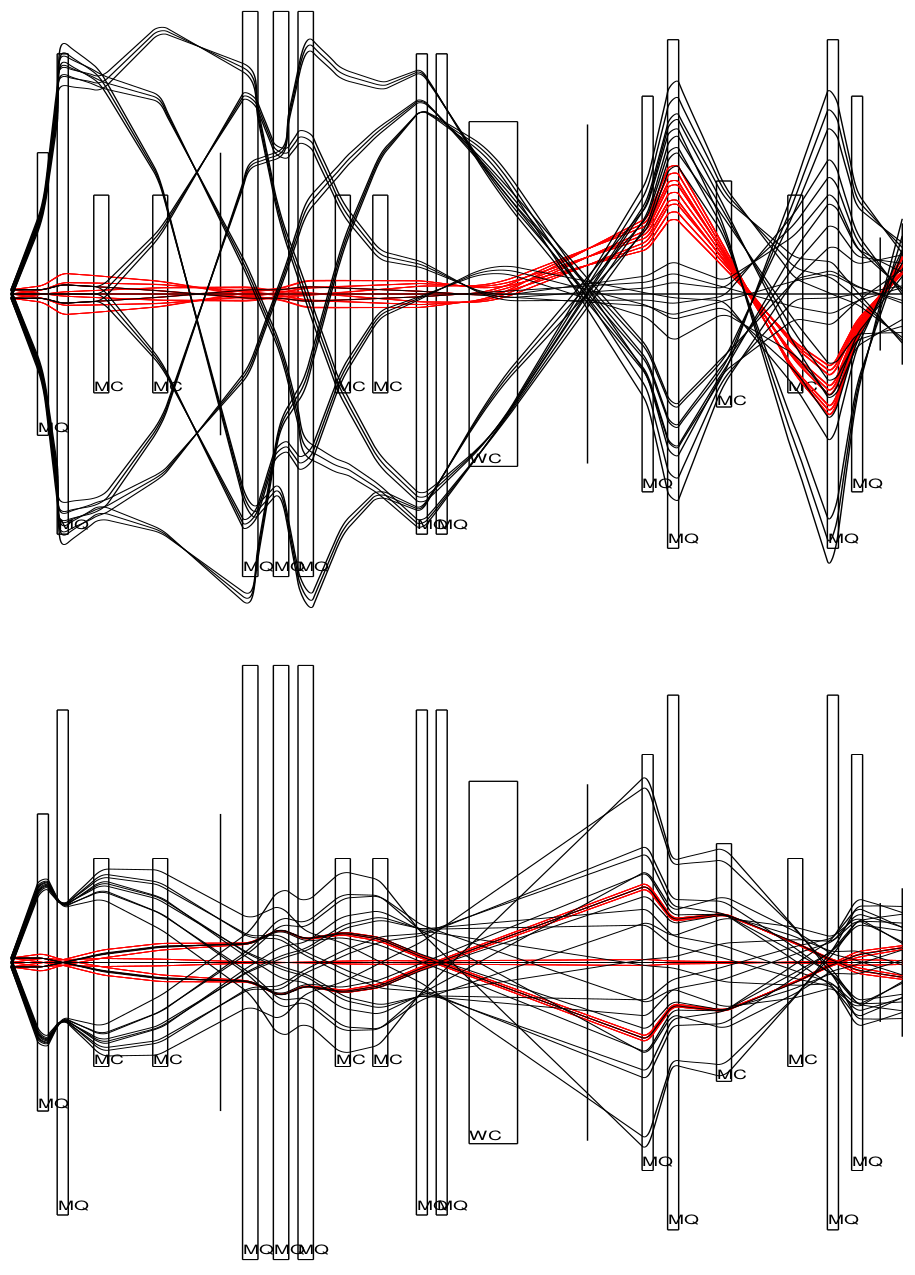
\includegraphics[width=0.8\textwidth]{figures/raytrace.png}}
        \caption[Horizontal and vertical rays through St.\
            George]{Horizontal (upper plot) and vertical (lower plot)
            rays through St.\ George. Recoil \nuc{41}{Sc} rays are shown
            in black and beam \nuc{40}{Ca} rays are shown in red.
            % The beam energy is $E_{\textrm{beam}} =
            % 15.99\pm0.001$~MeV, and the recoil energy is
            % $E_{\textrm{recoil}} = 15.6\pm1.155$~MeV.
            The beam rigidities are $B\rho = 0.331$~Tm and $E\rho =
            2.907$~MV, and the recoil rigidities are $B\rho = 0.331$~Tm
            and $E\rho = 2.836$~MV. Both the beam and recoil are in the
            $11^+$ charge state. Differing charge states would lead to a
            greater separation in the two beam profiles. The COSY
            calculation assumes that the recoil particles are spread
            within an acceptance range of $\Delta E/E \approx7.5$\,\%
            and $\Delta\theta = 40$~mrad. The transverse scale is highly
            exaggerated to show detail.}
        \label{fig:raytrace}
    \end{center}
\end{figure}


\section{Theoretical and Experimental Considerations}
\label{sec:cosy}

% Possibly move this to Chapter 2...

St.\ George was modeled using COSY Infinity (henceforth \emph{COSY}), a
beam optics and transport language developed at Michigan State
University~\cite{COSY}. The initial ion optics solution for the
separator was calculated by Drs.\ Couder and Berg at the University of
Notre Dame to maximize the angular and energy acceptance for a
point-like target located prior to the separator. Optimization of the
individual elements' properties allowed the separator to achieve the
previously-stated energy and angular acceptances, create an achromatic
focus at the mass slits (focal plane $F_2$), and transport all recoils
to the final detector focal plane $F_3$ (see Section~\ref{sec:stg}).
Each magnetic element is represented by a single command within the
code, defining the type and properties of the desired element. The three
types of elements used within St.\ George\----{}dipoles, quadrupoles,
and the Wien filter\----{}require different sets of values to be
defined. The recoil envelope, consisting of a number of sample recoil
properties used as representative rays, for the final designed
configuration is shown in Fig.~\ref{fig:raytrace}. For the example
shown, the quadrupole pole tip fields are given in
Table~\ref{tab:poletip}, where negative values represent a quadrupole
focusing in the $y$-direction. The pole tip fields for $(\alpha,\gamma)$
experiments are for the test particles shown, while those for $({\rm
p},\alpha)$ experiments are specific to this work. The actual fields
used will depend on the rigidity of the desired particle to transport
through the separator and can be scaled from these values.

The initial ion optics solution creates a transport map for particles
passing through the entire separator that can be analyzed independently
of the ray traces and provide the mathematical backing to the particles'
trajectories within St.\ George. The transport map is dependent on the
quantities

FIGURE OUT HOW TO CONDENSE THE COSY/BEAM OPTICS DISCUSSION INTO A SINGLE
SECTION (HERE OR INTRODUCTION)

\begin{equation}
    \label{eq:cosyvars}
    \begin{split}
        r_1 &= x \\
        r_3 &= y \\
        r_5 &= l = -(t - t_0)v_0\gamma/(1 + \gamma) \\
        r_7 &= \delta_m = (m - m_0)/m_0
    \end{split}
    \quad\quad
    \begin{split}
        r_2 &= a = p_x/p_0 \\
        r_4 &= b = p_y/p_0 \\
        r_6 &= \delta_K = (K - K_0)/K_0\\
        r_8 &= \delta_z = (z - z_0)/z_0,
    \end{split}
\end{equation}
where $a$ and $b$ are treated similarly to angles within each plane,
$\delta_K$ is the relative energy difference from the desired energy
$K_0$, $\delta_m$ is the relative mass difference from the desired mass
$m_0$, and $\delta_z$ is the relative charge from the desired charge
state $z_0$~\cite{COSY}. The desired quantities are the values used to
calculate the magnetic (Eq.~\ref{eq:brho}) and electric
(Eq.~\ref{eq:erho}) rigidity, and thus set the fields of the elements
within St.\ George, of the particle to be transported through the
entirety of the separator. The time of flight difference $l$ is not
considered in analyzing the separator. Within the transport map,
aberrations up to fourth order were calculated, with terms up to third
order found to affect the design~\cite{Couder2008}.

The original ion optics calculation describes the fringe fields of the
optical elements using the default parameters provided by COSY. A change
in the shape of the fringe field can change the trajectory of the
particles within the separator, as the total field that the particle
interacts with changes in magnitude. Since the fringe fields used to
find the ion optics solution and those created by the actual magnetic
elements within St.\ George may be different, the required field
strength may also be different. Additionally, the physical
electromagnetic elements produce fringe fields that may further differ
from the COSY design. Field maps for each of the magnetic elements were
produced by the production company in order to understand the dependence
of the field strength and fringe fields at differing excitations of the
magnet. The pole tip fields for a given particle rigidity, determined by
the current setpoint for that magnet, must be found experimentally. The
procedures for each of the three different types of elements necessarily
differ based on what diagnostic equipment is available.

The magnetic settings for the dipole magnets, determined by the rigidity
of the particles, can be determined by observing the trajectory of the
particles within the separator. This trajectory can be directly observed
using diagnostic equipment aligned with the optical axis. The search for
the required current powering the dipole magnet is then easier to
identify experimentally. The final setting of the dipole magnets must be
found by observing the effect of the focusing quadrupole magnets
following the dipole. If the beam is aligned with the magnetic optical
axis of the quadrupoles, the off-axis steering effects will be
minimized. This fine adjustment to the dipole fields is within a small
window of current settings for the dipole near the coarse value found
through direct observation of the beam.

Setting the Wien filter can be done in a similar manner. The electric
field strength is determined from the analyzed energy of the particle,
the known charge state, and the desired bending radius of the filter.
This bending radius is the radius of the particle's trajectory if only
the electric or magnetic field were operating. Thus, the electric field
strength can be set to an exact value, requiring the magnetic field to
be set to match the properties of the electric field. The strength of
the magnetic field is set such that the bending radii of the two fields
are the same and so that the particle beam continues along the optical
axis in the same manner as described previously with the standard
dipoles. The Wien filter was designed with magnetic field clamps at the
entrance and exit of the filter to match the magnetic field field to the
electric fringe field. These clamps must be adjusted to their proper
positions before the magnetic field can be set.

The magnetic quadrupoles require a more complex procedure in order to
set their fields to the desired values. This complication arises from
the inability to directly observe the trajectory of the focused
particles within the separator at all possible angles and energies
concurrently, and at multiple points within the separator itself. If
these trajectories match the trajectories expected from the beam optics
calculation, then the acceptance and rejection properties of the
separator would be the desired values. Due to the inability to do this,
the quadrupole tuning procedure must be adapted to work with the
diagnostic equipment available. The full procedure is outlined in
\ref{sec:tuning_stg}.


\section{Separator Properties}

% St George was installed the same year that I started grad school
The elements, power supplies, and supports were provided by Bruker
Biospin and installed in 2011. The separator design requirements for the
strengths of the optical elements were based on the maximum beam energy
of the older KN single-ended Van de Graff accelerator and the possible
charge states produced by its internal ion source. The 5U and ion source
have similar properties to this system. The power supplies for the
magnets provide highly stable direct currents for each magnet
individually, with $dI/I \approx 10^{-4}$ for the quadrupoles and $dI/I
\approx 10^{-5}$ for the dipoles. The upper current limit is different
for each magnet. The separator uses a robust water cooling system able
to maintain the required $80\pm2$~\degree{}F magnet temperature for the
entire system. The system is able to maintain the temperature even when
all magnets are at their maximum currents for extended periods of time.

The Wien filter electrode power supplies are set separately based on
their voltage, with voltage stability $dV/V \approx 10^{-5}$ in the
range commonly used for experiments. The upper limits for these power
supplies are $\pm110$~kV, with voltages below $\approx 70$~kV used
during previous work. In order to reach voltages near the top range, the
voltages need to be slowly ramped up to ``condition'' the plates at the
higher voltage. This conditioning is required due to minor imperfections
on the surface of the electrostatic plates, differences in the residual
vacuum within the vacuum chamber, and buildup of C deposits on the
plates and interior walls. Directly setting the plates to higher
voltages without conditioning the plates would lead to large and
frequent discharges of the electrostatic plates, preventing the Wien
filter from being used in stable running conditions. For voltages above
$\approx 50$~kV, the plates were conditioned to voltages at least 10~kV
above the desired setpoint to provide a stable running condition. For
lower voltages, no conditioning is necessary unless the vacuum chamber
was recently vented (exposed to atmospheric pressure gases).

The properties (entrance and exit apertures, length, maximum field
strength, good field region, etc.) were determined within the ion optics
solution to transport the desired recoils, and built to match those
specifications. Higher order corrections to the particle trajectory were
achieved by shaping the entrance and exit faces of the dipoles instead
of using higher order multipole magnets~\cite{Couder2008}. Additionally,
the shape of the Wien filter electrostatic plates were designed such
that the electric and magnetic fields, including the fringe fields, were
closely matched.


\subsection{Magnetic Fringe Fields and Effective Field Lengths}

Detailed two-dimensional magnetic field maps for multiple excitations of
each magnet were provided by Bruker. The field maps allow a check on the
good field region for each magnet and provide a description of the
fringe fields. Field strengths at each location (distance along the beam
axis and at a radial distance from the beam axis) are measured in mT.
From this data, the shape of the fringe field and the effective field
length of the magnetic elements can be determined. The effective field
length, defined as
\begin{equation}
    \label{eq:efl}
    L = \frac{1}{B_0}\int_{-\infty}^{\infty} B(z)\, \textrm{d}z,
\end{equation}
where $B_0$ is the field strength at the center of the magnet, is the
field length if the field were described with a pure ``hard edge'' or
Heavyside function at the entrance and exit, i.e.\ no fringe fields. As
these values are essential to setting the necessary values for the
quadrupoles, the analysis of the field maps focused on these elements.

A single edge fringe field is described by the Enge function given by
\begin{equation}
    \label{eq:enge}
    E(z) \equiv \frac{1}{1 +
        \exp\left[\sum_{i=0}^{N-1}{a_i}(\frac{-z}{D})^{i}\right]},
\end{equation}
where $a_i$ are the desired expansion coefficients, $D$ is the aperture
diameter, and $z$ is the longitudinal distance~\cite{Baartman2007}. The
formulation above is used within COSY to describe user-defined fringe
fields. For a short magnet, which the St.\ George quadrupoles can be
considered to be, the entrance and exit fringe fields are not completely
independent of each other, since the fringe fields extend into the
central region of the magnet. Instead of fitting each fringe field
separately, we can instead fit the entirety of the magnetic field
profile using a combined ``short'' quadrupole function, in terms of the
Enge function, given by
\begin{equation}
    \label{eq:shortquad}
    k(z) = k_0\left[E(L/2 + z) + E(L/2 - z) - 1\right],
\end{equation}
where $k_0$ is a scaling parameter for the central field and $L$ is the
effective field length~\cite{Baartman2007}. This formulation assumes a
symmetric field profile, as both the entrance and exit fringe fields are
modeled with the same Enge function.

\begin{figure}[t]
    \begin{center}
        \centerline{
            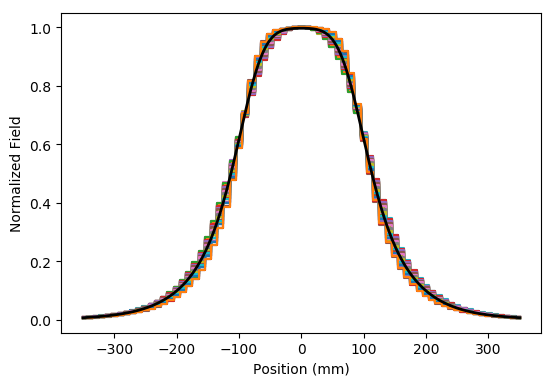
\includegraphics[width=0.85\textwidth]{figures/enge_fit.png}}
        \caption[Normalized field with Enge fit]{Normalized field and
            the resultant fit to the fringe field for the example
            quadrupole $Q_{10}$. The parameters of the fit are given in
            Table~\ref{tab:enge}.}
        \label{fig:enge_fit}
    \end{center}
\end{figure}

Using the field maps provided by Bruker, we can determine the Enge
coefficients and the effective field lengths for our magnets. For all
calculations, since the field near the center of the magnet is
relatively weak, the fields within 2~cm in the radial direction of the
central axis were not used for determining either the effective field
length or the Enge coefficients. Additionally, the effective field
length and the shape of the fringe field were assumed to not differ with
different magnet excitations, so all available data were used for each
magnet at the same time. An example using $Q_{10}$ of the normalized
fields used and the resulting fit is shown in Fig.~\ref{fig:enge_fit}.

The effective field lengths were calculated directly from the field maps
by integrating along the $z$-direction for each radial distance
provided. Since the maximum field strength for a given magnet current
varies depending on the distance from the center, the individual
``traces'' of the magnetic field along the $z$-axis were normalized.
This normalization is shown in Eq.~\ref{eq:efl} as the constant factor
outside of the integral. The integration was performed using the
Simpson's Rule routine provided by the SciPy Python
package~\cite{SciPy}. An average of these lengths was used. Differences
between the calculated effective field length and those used within the
initial ion optics solution were within 2\,\%.

Using the same normalized field ``traces'' along the $z$-axis, the Enge
coefficients describing the shape of the fringe field may be determined.
The field profiles at each radial distance were fit simultaneously.
Using the default Enge coefficients as the initial parameter guesses,
the summed mean squared error between the data and
Eq.~\ref{eq:shortquad} was minimized using the Nelder-Mead downhill
simplex minimization (see \cite{Simplex}) provided by
SciPy~\cite{SciPy}. The additional factor $k_0$ was included in the fit,
but is not needed when defining a fringe field within COSY. The process
was repeated for each quadrupole separately. The updated Enge
coefficients and their comparison to the default values used by COSY for
$Q_{10}$ can be seen in Table~\ref{tab:enge}, and the difference in the
shape of the fringe field can be seen in Fig.~\ref{fig:enge_comparison}.

\begin{table}[t]
    \begin{center}
        \caption{ENGE COEFFICIENTS FOR $Q_{10}$ COMPARED TO COSY DEFAULTS}
        \label{tab:enge}
        \begin{tabular}{c S[table-format=2.8]S[table-format=2.6]}
            \toprule
            \midrule
            \textbf{Coefficient} & \textbf{$Q_{10}$ Values} &
                \textbf{COSY Defaults} \\
            \midrule
            $k_0$ &  0.99731489 & \\
            $a_0$ &  0.37255261 &  0.296471 \\
            $a_1$ &  6.18699778 &  4.533219 \\
            $a_2$ & -5.55514115 & -2.270982 \\
            $a_3$ &  6.96210851 &  1.068627 \\
            $a_4$ & -4.82581328 & -0.036391 \\
            $a_5$ &  1.3135787 &  0.022261 \\
            \bottomrule
        \end{tabular}
    \end{center}
\end{table}

\begin{figure}[t]
    \begin{center}
        \centerline{
            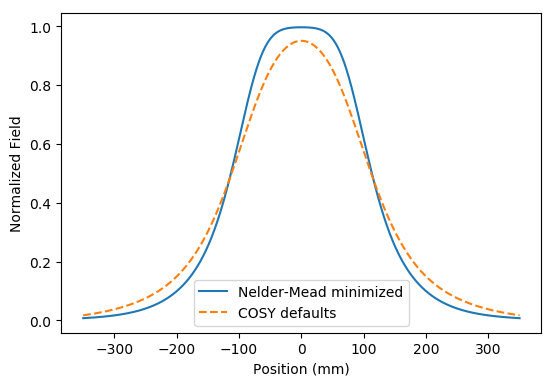
\includegraphics[width=0.85\textwidth]{figures/enge_comparison.png}}
        \caption[Comparison between fringe fields]{Comparison between
            fringe fields for the example quadrupole $Q_{10}$. The COSY
            default parameterization for the fringe field is the dashed
            orange line, and the fitted fringe field is the solid blue
            line. The distinct difference between the two field
            characterization requires the higher order effects arising
            from the fringe field to be taken into account.}
        \label{fig:enge_comparison}
    \end{center}
\end{figure}

In some cases, the field maps were not recorded far enough away from the
center of the magnet for the fitting routine to converge, primarily due
to the field not adequately reaching zero. In those cases, ``dummy''
points of zero field were pre\---{} and post\---{}pended to the
individual ``traces'' at distances greater than 5~m from the center of
the magnet to aide in convergence.

The default COSY coefficients for the fringe field were compared against
the data and shown to not adequately describe the field maps. The summed
mean squared error when using the short quadrupole formalization and the
default COSY parameters was significantly larger than that found through
the minimization routine, and the difference was shown to be
statistically significant. A visual comparison between the two models
for $Q_{10}$ is shown in Fig.~\ref{fig:enge_comparison}.

These new terms describing the effective field length and the fringe
field can be used to provide a more realistic beam optics solution for
St.\ George. To create this realistic solution, the magnetic fields of
the various elements within the separator were redefined with these
newly found values. The beam optics solution was refit by minimizing a
cost function defined in terms of our desired transfer matrix properties
at our focal planes, such as the mass and energy dispersion at the
post-Wien filter focal plane $F_2$, the beam spot size at the final
detector plane $F_3$, and other properties. From this recalculated
solution, new pole tip fields for the focusing quadrupoles are
determined which can provide a more accurate estimate of the actual
experimental field required for the experiment.


\section{Energy and Angular Acceptance}
\label{sec:commissioning}

The energy and angular acceptances of St.\ George were determined
experimentally through a series of experimental campaigns using multiple
rigidities. The energy acceptance without a corresponding angular
acceptance was shown to exceed the designed acceptance at zero degrees,
with a measured energy acceptance of $\Delta E/E = \pm 8$\,\% for ten
different beam rigidities covering the phase space region for
astrophysically important recoils~\cite{Meisel2017}. The angular
acceptance has been shown to meet the desired $\Delta\theta = \pm
40$~mrad in limited cases with an energy spread of $\Delta E/E = \pm
3$\,\%. The full total acceptance has not yet been measured within the
designed phase space limits of St.\ George, with work ongoing.

Within the following discussion, the term ``test beam'' will be used in
reference to an incident beam produced by the 5U with a desired
rigidity. These test beams are defined by the selected beam particle,
energy, and charge state, which determines the magnetic and electric
rigidity. Test beams with different rigidities were chosen to adequately
cover the possible rigidity phase space during the commissioning
experiments (see Fig.~\ref{fig:rigidity-phase-space}). These beams were
chosen for to provide particles with the desired rigidity and with beam
currents in the range of $0.5 - 3$~$\mu$A in order for the diagnostic
equipment to properly measure the beam. Additionally, those beams that
commonly had highly stable 5U and ion source running conditions over
extended times were selected to reduce beam preparation steps by the
operators.

Acceptance measurements first probed the energy acceptance within the
designed $B\rho-E\rho$ phase space. The rigidity phase space limits,
along with measured acceptances and ranges for proposed future
experiments is shown in Figure~\ref{fig:rigidity-phase-space}. The
regions of astrophysical interest are accessible by various test beams
that can be produced by the 5U, allowing the phase space to be
adequately studied.

\begin{figure}[t]
    \begin{center}
        \centerline{\includegraphics[width=0.8\textwidth]%
            {figures/rigidity_phase_space.png}}
        \caption[Designed $B\rho-E\rho$ rigidity phase space for St.\
            George]{Designed $B\rho-E\rho$ rigidity phase space for St.\
            George. Stars represent rigidities that have been shown to
            have the full $\Delta E/E = 8$\,\% energy acceptance.
            Reactions shown are probable first experiments using St.\
            George that use beam energies accessible with the 5U:
            \nuc{14}{N} at $E_{\rm{beam}}\approx 0.7-5.0$~MeV (solid
            blue line), \nuc{3}{He} at $E_{\rm{beam}}\approx
            0.25-1.2$~MeV (dashed orange line), and \nuc{12}{C} at
            $E_{\rm{beam}}\approx 3.0-10.0$~MeV (dotted green line).
            These energy ranges cover some of the astrophysically
            important ranges for the given reactions. Adapted
            from~\cite{Meisel2017}.}
        \label{fig:rigidity-phase-space}
    \end{center}
\end{figure}


\subsection{Beam Tuning and Properties}
\label{sec:tuning}

The commissioning runs followed a similar procedure for beam preparation
using the 5U and the transport line. The beam rigidities were chosen to
cover a region within the phase space limits of the separator that cover
recoils produced through reactions of astrophysical interest. Both light
(\nuc{1}{H} and \nuc{4}{He}) and heavier (\nuc{16}{O} and \nuc{20}{Ne})
beams were used to probe different regions of that phase space. Angular
acceptance runs to date have only used lighter beams. The energy
uncertainty of the beam is approximately 0.3~keV, and a conservative
value of 0.5~keV will be used when necessary.

Beam preparation can be divided into two segments: preparing the $\Delta
E = 0$ test beam to enter into St.\ George along the central magnetic
optical axis, and transporting that beam along the central magnetic
optical axis within St.\ George. The following procedures were used for
all acceptance measurements, with differences being minor. The
diagnostic equipment described in Section~\ref{sec:diagnostic} was
essential to performing the beam preparation steps and their use is
highlighted below.

\subsubsection{Before St.\ George}

Test beam preparation before St.\ George is required to prepare the beam
for the experimental requirements of the commissioning runs: the beam
\begin{enumerate}
    \item must enter along the magnetic optical axis;
    \item must have a narrow waist point with circular cross section at
        the target location;
    \item must have a focus that is not highly divergent; and
    \item must be stable with low energy uncertainty and relatively high
        current.
\end{enumerate}
These requirements are fulfilled through the operation of both the 5U
and the transport beam line, with the last two requirements primarily
beneficial from an experimental standpoint. The beam divergence is the
maximum angle of the particle trajectory caused by the focusing elements
along the transport line, and is related to the magnetic fields used to
focus the beam and the properties of the beam, such as beam extent and
rigidity. A graphical description of these dependencies is shown in
Fig.~\ref{fig:divergence}.

\begin{figure}[t]
    \begin{center}
        \centerline{\includegraphics[width=0.8\textwidth]%
            {figures/quad_focus_divergence_2.png}}
        \caption[Sketch of beam divergence due to focusing
            strength]{Sketch of the beam divergence caused by the
            focusing strength of a quadrupole magnet. Increasing
            darkness corresponds to increasing strength of the magnetic
            field. When focusing in a single direction, the apparent
            beam spot (shown on the right) must diverge in the other
            direction. The requirements of the tune will determine what
            beam shape some distance from the quadrupole is required.}
        \label{fig:divergence}
    \end{center}
\end{figure}

The chosen beam intensity is dependent on which diagnostic equipment
will be used. The isolated Faraday cups cannot read current below
50~$e$nA when read through the logarithmic amplifier at the console, and
the current can't be above 20-30~$e\mu$A as the cups are not currently
water cooled and a high intensity and focused beam may melt some of the
components. This upper current limit was not approached during the
tests, since the cups were used in tandem with the quartz viewers. The
quartz viewers are limited to beam currents of a maximum of 3-5~$e\mu$A,
as higher currents risk heating up the quartz to a high enough
temperature to cause them to shatter or melt. Since four of the quartzes
are also barriers between the high ($10^{-8}$~torr) vacuum within St.\
George and atmosphere, this limit must be carefully avoided. In
practice, currents between 500~nA and 4~$\mu$A were used, based on the
exact properties of the ion source for that particular run, the beam
species, and the locations of slits on the primary transport line used
to reduce the beam current.

The procedure for aligning the test beam to the magnetic optical axis is
described below. Major subsections of the procedure will begin with a
short title in bold to guide the reader. The elements on the main
transport line that may be necessary to adjust are the switching magnet
with the $X_6$ steerer, and the $Y_5$ and $Y_6$ steerers (locations
shown in Figure~\ref{fig:5U}). The steerers are labeled as such based on
their position along the main transport line. Steerers $X_6$ and $Y_6$
are part of the same physical steerer but can be operated independently.
Additionally, the quadrupole triplet directly before the target location
will be necessary for final tuning.

\textbf{Aligning the beam to St.\ George's optical axis:}
The desired test beam is transported down the St.\ George transport line
and monitored with the Faraday cup at the target location, called the
\emph{target cup} for beam current stability. Diagnostic equipment
before the target location are used as an aide to transport the beam and
ensure that it has the desired properties. If necessary, the beam
current is reduced. The quadrupole triplet is not used at this point,
since the beam may not be entering the element along its magnetic
optical axis.

The beam is sent into St.\ George. With no field in $Q_1$, $Q_2$, and
$B_1$, the beam hits the quartz viewer at the 0\degree{} exit port of
the magnetic vacuum chamber, called the \emph{$B_1$ quartz}. If the beam
does not strike the quartz, then the final set of steering elements
needs to be adjusted to send the beam into the quartz.

\textbf{Checking for steering:}
Quadrupoles $Q_1$ and $Q_2$ are adjusted independently of each other,
and the resulting motion of the beam on the quartz is recorded. If the
beam is aligned with the central magnetic optical axis, the quadrupole
will only focus the beam and not shift its position on the quartz, i.e.\
the spread in the beam will change but not its central position. The two
quadrupoles must be adjusted independently of each other as any induced
steering from a beam misalignment in one may be counteracted by a
misalignment in the other quadrupole. If the beam is steered by either
quadrupole, the steering elements preceeding the offending quadrupole
are adjusted to reduce that steering. Commonly, the elements that steer
in the same direction as the focusing direction of the quadrupole (i.e.\
$Y_5$ and $Y_6$ for $Q_1$, the switching magnet and $X_6$ for $Q_2$)
will provide the largest improvement to the steering. Minor corrections
to all preceeding steering elements may be required as the non-steering
solution is approached.

A quadrupole steers a beam when the beam enters the magnetic element
misaligned with the optical magnetic axis. Assuming that the element is
brought from zero to defined strength, the focal length of the
quadropule changes from $\infty$ to a length $f$. The effect on the beam
is that those regions of the beam away from the optical axis are brought
to pass through this focal point. When a beam is aligned with the
magnetic optical axis, there is an equal amount of the beam on either
side of this optical axis, so the beam spot will narrow along the
focusing axis of the quadrupole. The beam will also extend along the
other axis. If the beam is not aligned with the optical axis, this beam
motion to the focal point will be viewed as a lateral motion along the
focusing axis of the quadrupole. A sketch of this effect can be seen in
Figure~\ref{fig:steering}.

\begin{figure}[t]
    \begin{center}
        \centerline{\includegraphics[width=0.8\textwidth]%
            {figures/quad_steering_2.png}}
        \caption[Sketch of quadrupole steering of misaligned
            beam]{Sketch of the steering caused by a quadrupole magnet
            due to the beam being misaligned to the magnetic optical
            axis. Increasing darkness corresponds to increasing magnetic
            field strength. From the misalignment, the beam spot appears
            to move along the focusing axis at some distance. The
            scanning motion of the spot can be used as a diagnostic
            tool to determine the beam alignment. If the beam spot is
            not moving in the focus direction as the magnetic strength
            is changed, the beam is aligned to that quadrupole's
            magnetic axis.}
        \label{fig:steering}
    \end{center}
\end{figure}

The goal for adjusting the steering elements before St.\ George is to
have each quadrupole induce no steering on the beam. In practice, each
change to the steering elements either increases or decreases the amount
of steering in the direction of that element. The crossover point, where
the beam switches from steering left to steering right for example, can
be used to restrict the possible phase space of steerer values, as the
beam must have a zero deflection position between those two extremes.

A single quadrupole may induce steering in both directions based on the
beam conditions. For example, a beam that is misaligned in both the $+x$
and $+y$ direction entering into a quadrupole focusing in the $y$ plane
will be steered in both the $+x$ and $-y$ direction. When minimizing
steering in a single direction, the other direction must be periodically
checked to ensure that a minimal steering solution is reached for both
directions at the same time.
%
At the end of this process, the beam is not deflected when the field
strength for either $Q_1$ or $Q_2$ is increased or decreased
independently of the other quadrupole. The beam may be said to be
entering St.\ George along the optical magnetic axis. Due to the short
distance between the first quadrupole doublet and the $B_1$ quartz, it
may be necessary to increase the sensitivity of the steering to ensure
that we are as aligned as possible to the axis.

\textbf{Increase sensitivity:}
The beam is then sent further into St.\ George, first to the $B_2$
quartz located within the beamline then the $B_3$ quartz. The steering
of $Q_1Q_2$ is again checked in the same fashion as before. As these
quartzes are located further from the quadrupoles, they give a higher
sensitivity to steering effects from misalignment than just using the  % check effects/affects for this case
$B_1$ quartz at the trade-off that the the quadrupoles can only be set
to lower field strengths. Since the quartz is further from the focusing
elements, the same focusing strength will create a larger beam spot on
the quartz viewer. This effect can be seen in Figure~\ref{fig:steering}.

These additional checks require $B_1B_2$ to have field. While these two
dipoles must have an exact field strength when performing acceptance
measurements or an experiment, at this point their fields only need to
be coarsely set such that the beam strikes the desired quartz. While the
higher order corrections from these magnets do play a role in the
direction and focusing of the beam, that contribution has no effect on
determining beam alignment within the quadrupoles.

The steering elements are adjusted in the same fashion to minimize
steering in $Q_1Q_2$. Since this steering was minimized during the
previous step, these adjustments should be minimal. It may be necessary
to have a weak field in $B_3$ in order to see the beam on the $B_3$
quartz, due to possible machining misalignments of the port that the
quartz is attached to and the residual magnetic field within the dipole.

\textbf{Include the quadrupole triplet:}
As the last focusing element before St.\ George, the quadrupole triplet
(henceforth simply the \emph{triplet}) is the final adjustable element
to determine the beam properties when entering the separator. The
triplet is used to focus the beam to a small spot at the target
location, a requirement for both experiments and acceptance
measurements. As it and $Q_1Q_2$ should lie on the same magnetic optical
axis, its steering must also be checked and minimized if its use is
desired for the present experiment. It was not used in all cases as the
coarse target focus provided by the previous quadrupole doublets on the
main transport line were deemed sufficient.

Before moving the beam off of the $B_1$ quartz, the steering effects of
the triplet must be characterized in the same fashion as $Q_1Q_2$.
During the steering minimization steps, both the triplet and $Q_1Q_2$
must both be minimally steering before moving forward.

Due to minor misalignments between the triplet and $Q_1Q_2$, it is
usually not possible to have all elements nonsteering at the same time.
In these cases, the steering of $Q_1Q_2$ should take precedence while
having the triplet minimally steering. While the steering of the beam
prior to the target location is important, experimentally the steering
of the individual elements within the triplet cancel or nearly cancel
each other out when the triplet is minimally steering, reducing that
problem.

At this point, the main transport line has been tuned to prepare a
well-focused and well-aligned beam entering into St.\ George. These
elements are not to be touched during the rest of the tuning process.
The triplet, due to the possibility of it having minor steering effects,
must also have zero field for the remainder of the steering checks, and
will be turned on for the actual measurement.

\subsubsection{Within St.\ George}
\label{sec:tuning_stg}

Once the test beam has been aligned to enter the separator along the
magnetic optical axis, it must also be aligned to the magnetic optical
axes of all of the quadrupoles within the separator. This alignment is
done using only the dipoles $B_{1-6}$ and the WF. Any minor misalignment
in the vertical direction should have been corrected during the previous
steps, but there is the possibility that there will be vertical steering
within the separator, both from that misalignment and effects from the
dipoles and quadrupoles. The procedure for this second alignment is
straightforward, as the only elements used to adjust the steering of the
quadrupoles are the two dipoles immediately prior.

\textbf{Tuning to the WF:}
With the beam striking the $B_3$ quartz, quadrupoles $Q_{3-5}$ are
checked for steering. The primary focus of these steering checks will be
on $Q_3$ and $Q_5$ which focus in the horizontal plane. The magnetic
fields within $B_1B_2$ are adjusted to make these quadrupoles
non-steering or minimally steering. The field precision is on the order
of 0.1~G, read back by the Hall probes.

Due to potentially small misalignments in the St.\ George quadrupoles in
relation to each other, it is commonly not possible to have $Q_{1-5}$
non-steering simultaneously (see \cite{Meisel2017}). In these cases,
minimal steering can be achieved through $Q_{3-5}$ by adjusting $B_1B_2$
when $Q_1Q_2$ are non-steering. At this point, dipoles $B_1B_2$ are set
to the value corresponding to the magnetic rigidity of the particle and
to maintain the test beam alignment to the optical axis.

Dipoles $B_3B_4$ are brought up to their rough field value to send the
beam through the WF and onto either the WF quartz or the $B_5$ quartz.
The quadrupoles $Q_{6-9}$ are checked for steering, adjusting $B_3B_4$
to minimize the steering. The focus at this point is on getting a
non-steering solution for $Q_6Q_7$, as $Q_8Q_9$ can also be corrected by
the Wien filter. Since there is some residual magnetic field within the
Wien filter, the electric field is brought up to compensate for this
bending to keep the test beam along the optical axis through $Q_8Q_9$.
The field required is calculated by determining the bending radius
caused by the residual magnetic field and creating the equivalent
bending radius in the opposite direction for the particle's $E\rho$.

As the beam envelope has expanded, it will be necessary to bring
$Q_{1-5}$ to their desired values in order to check the steering of the
remaining quadrupoles. Since these quadrupoles have been shown to be
minimally steering, their effect on the beam trajectory through the
remainder of St.\ George should be negligible. It may be necessary to
have a weak field in $B_5$ in order to see the beam on the $B_5$ quartz
for the same reasons as explained previously for $B_3$.

\textbf{Setting the WF:}
For a test beam with $\Delta E = 0$ and $\Delta\theta = 0$, the elements
within St.\ George will be set to transport this along the central axis
based on the test beam's rigidity. Since the energy of the beam is well
known and the charge of the beam is exact, the electric rigidity $E\rho$
is also well known when tuning for a set bending radius. For St.\
George, the Wien filter bending radius is $\rho_{\rm WF} = 4.348$~m. The
electric dipole within the WF is set for this rigidity and held constant
for the remainder of the tuning process.

The magnetic field is set similarly to the other dipoles: to minimize
the steering induced by the next set of quadrupoles ($Q_8Q_9$). Since
the test beam was aligned to the optical magnetic axes of this
quadrupole doublet in the previous step, the WF magnetic dipole must
return the beam to this orientation. The preceeding magnetic quadrupoles
$Q_{1-7}$ must also be set to their required values. These values are
found by scaling the calculated tune based on the rigidity of the test
beam; in cases where an optimal solution was found experimentally that
differs from the COSY calculated values, those \emph{in situ} optimized
values are used as the baseline. The quadrupoles are required to be set
since the elements within St.\ George up to and including the Wien filter
work to separate the beam particles by mass, so setting them mimics the
situation during an experiment.

The magnetic field for the WF is read back using a Hall probe located on
the pole face. The field can be set precisely and related to the fields
in the other dipoles. Once the magnetic field is set such that $Q_8Q_9$
do not steer the beam, the full WF is set.

\textbf{Tuning through the detector chamber:}
Dipoles $B_5B_6$ are set to their rough values based on the $B\rho$ of
the test beam, sending the beam through the detector chamber and onto
the last quartz, called the \emph{detector quartz}. As before, due to
the size and shape of the beam envelope, $Q_8Q_9$ must be set to the
required values. The final two quadrupoles $Q_{10}Q_{11}$ are checked
for steering, and $B_5B_6$ are adjusted to minimize that steering.

Since the test beam is traveling through the detector chamber, the
entire detection system must be pulled out of the way of the beam.
Magnetic shields have been placed below the MCP constructs to remove the
effect of the magnetic fringe fields on the beam
deflection~\cite{MoralesDNP}. Once $Q_{10}Q_{11}$ are non-steering, the
test beam is fully aligned to the optical magnetic axis of St.\ George.

\subsubsection{Collimator and Target Position}

The 2~mm diameter collimator at the target location (see
Section~\ref{sec:target}) is used for setting the triplet to the proper
values. A narrow waist beam at the target location is a requirement to
achieve the maximum angular and energy acceptance for St.\ George. With
the collimator in place, the triplet is adjusted such that the beam
transmission, defined as the ratio between the beam currents before and
after the collimator as read by two separate Faraday cups, is maximized
and ideally close to 100\,\%.

Since the target chamber may rotate around its central axis, it is
possible for the location of the collimator to become slightly
misaligned between runs. Additionally, the triplet may induce some minor
steering at the target location, potentially moving the focal point
radially from the optical magnetic axis. The target collimator position
is then not a fixed value but must also be tuned to maximize
transmission. Once the collimator position is found, the target position
is immediately known. Empirically, a small range of possible values for
the rotation and extension of the target ladder have been found to be
optimal, restricting the search space when tuning.

For acceptance measurements, the collimator is used to create a focal
point at the target location. Once the beam preparation is complete, it
is retracted from the beamline. In situations where a target foil is
used as a ``degrader'' to provide an angular and energy spread, the
relative distance between the collimator and the foil is used to
properly align the foil to the beam.

\subsubsection{Additional Considerations}
The steering minimization routine can never fully eliminate the beam
steering because of possible misalignments of the magnetic elements and
the properties of the beam. Especially of concern would be the vertical
steering of the $y$-focusing quadrupoles ($Q_{1,\,4,\,7,\,8,\,11}$), as
the alignment of the beam to their axis is primarily affected by the
beam preparation steps before the beam enters St.\ George. These
quadrupoles may steer minorly in the vertical direction despite the best
efforts of the operator. As there are no elements within St.\ George
that could correct for this, the steering effect of these quadrupoles
may not be able to be eliminated.

As the process is repeated, the required field strengths for the magnetic
dipoles within St.\ George will be better known, and additional global
settings for St.\ George

\subsection{Energy Acceptance}

The energy acceptance of St.\ George at $\Delta\theta = 0$~mrad was
measured to be $\Delta E/E = \pm 8$\,\% for ten different rigidities
(see Fig.~\ref{fig:rigidity-phase-space} and \cite{Meisel2017}). The
measurements took place before angular acceptance target chamber was
built and will be remeasured as part of a total acceptance measurement
campaign. Test beam rigidities were chosen to cover an adequate region
within the designed phase space near the rigidities expected for recoils
of astrophysical interest and based on the restrictions imposed by the
5U and ion source.

For a given set of field settings for a test beam at $\Delta E = 0$ that
provide 100\,\% transmission between the target cup and a Faraday cup
located within the detector chamber at focal plane $F_3$, the separator
is said to accept an energy difference if the test beam is changed to
that different energy and still have 100\,\% transmission between those
two cups. To state that St.\ George has an energy acceptance of $\Delta
E/E = \pm 8$\,\%, a single set of fields for the elements within the
separator transmitted 100\,\% of the test beam between the two cups when
its energy was changed within that energy change.

The procedure for measuring the energy acceptance of a single rigidity
is outlined below. The slits located at the post-WF focal plane $F_2$
were used to define a beam center. As the tune for a given recoil is
supposed to be achromatic at this location, these slits were used as
both a diagnostic on the path of the beam and a check of this
requirement during the measurements. Note that the tuning process for
these measurements did not make use of the in-beam quartz viewers at
$F_1$ and $F_2$ since they had not yet been installed.

\textbf{Initial setup:}
After tuning a beam along the optical magnetic axis as described in
\ref{sec:tuning}, all elements within St.\ George are at a given field.
The dipole elements, including the WF, are not touched. The transmission
between the target cup and the $F_3$ cup is measured. If the
transmission is 100\,\%, the beam energy was changed. If not, then the
quadrupoles were retuned to transmit 100\,\% of the test beam between
the two cups.

Quadrupole retuning was done systematically to prevent over- or
under-focusing the beam at any location within St.\ George. With the
beam on the $F_3$ cup, each quadrupole was adjusted individually to
determine what field is required to transmit 100\,\% of the beam to the
cup. After finding that field, the difference is recorded and the
quadrupole is returned to its original value. This process is repeated
for every quadrupole acting independently. If a single quadrupole could
not achieve 100\,\% transmission on its own, it was not included in the
next step. Assuming $N$ quadrupoles adjusted by $\Delta B_i$ to give
100\,\% transmission, the individual quadrupoles $Q_i$ were changed by
$\Delta B_i / N$. This approach usually resulted in achieving 100\,\%
transmission for the $\Delta E = 0$ case.

The quadrupole adjustment described was used at every step if the tune
was shown to not transmit 100\,\% of the test beam. Previous settings of
the quadrupoles were recorded to map regions of field strengths were
100\,\% transmission was achieved for different energy changes.

\textbf{Changing energy:}
The beam energy was changed to $\Delta E/E = -8$\,\% by changing the
accelerator. The transport beamline was scaled automatically to account
for the change in rigidity. The beam was shown to enter into St.\ George
along the optical magnetic axis by putting the fields within $Q_1$,
$Q_2$, and $B_1$ to zero and checking the steering of the first two
quadrupoles. Since this energy change is minor, in most cases only the
switching magnet needed to be changed. The magnets $Q_1Q_2B_1$ were
brought back to their required values and transmission between the two
cups was checked.

If the beam was fully transmitted to the $F_3$ cup, the settings for
St.\ George were said to have an energy acceptance of $\Delta E/E =
-8$\,\%. The beam energy was then changed to $\Delta E/E = + 8$\,\%,
following the same procedure, and transmission was checked. If the beam
also was fully transmitted, the separator tune was said to have an
energy acceptance of $\Delta E/E = \pm 8$\,\% and the measurement was
complete.

Where 100\,\% transmission was not achieved, the quadrupole scaling
described previously was used. The new tune was recorded, and the beam
energy was returned to $\Delta E = 0$ to check transmission. This
process was continued until all three energy points had 100\,\%
transmission for a single setting of St.\ George. During this cycling,
referring to previous values was used to prevent correcting the tune in
one direction at one energy only to change back to the previous tune at
another energy.

Since the $F_2$ slits were placed around the beam center, achieving
100\,\% transmission was only possible if test beam had a nearly or
completely achromatic focus following the WF, one of the requirements
for normal operation of the separator.

\textbf{Additional measurements:}
For subsequent energy acceptance measurements, instead of using the COSY
predicted values, an energy acceptance tune scaled based on the magnetic
rigidity $B\rho$ of the new test beam was used for the initial
quadrupole settings. If the difference in $B\rho$ was sufficiently
small, the required adjustments to the quadrupole fields were minimal,
speeding up the measurement process. As more individual energy
acceptance measurements were made, the scaling based on $B\rho$ became
more robust to slight differences in beam preparation and species.

Once the ten rigidities within the astrophysically interesting phase
space of the separator were measured, work moved to measuring the
angular acceptance.


\subsection{Angular Acceptance}

As of this writing, the angular acceptance of St.\ George has been
measured to be $\Delta\theta = \pm 40$~mrad in the horizontal and
vertical planes for a single rigidity. The acceptance was shown by
ensuring 100\,\% transmission when deflecting the beam 40~mrad in each
direction, and quadrupole adjustments followed the same procedure as
during the energy acceptance measurements. The measurement was done
without a corresponding energy acceptance, and without the requirement
that the test beam be focused at the focal plane $F_2$ following the WF
and without the beam passing through the slit opening at that location
for all deflection angles. The measurement was then a single ``proof of
concept'' that an angular acceptance could be measured using the new
diagnostic and control equipment installed. Due to complications with
the measurement process, multiple attempts at measuring the angular
acceptance, each with a different procedure, were tried. These attempts
are outlined below.

\textbf{Deflector plates only:}
A test beam is tuned to provide a non-steering beam with 100\,\%
transmission between the target and $F_3$ cups. The deflector plates
(see Section~\ref{sec:target}) are rotated so that they deflect the beam
in a single plane. The horizontal plane was commonly chosen first. Since
the entrance aperture for the target cup is larger than 40~mrad, it does
not intercept any of the beam when it is deflected. Angles between 0 and
40~mrad were used and the current on the $F_3$ cup was monitored. The
maximum angle that provided 100\,\% transmission was recorded.

If the maximum angle achieved was not 40~mrad, the quadrupoles were
tuned in the same fashion as for the energy acceptance measurement but
with the deflector plate set to an angle greater than was accepted such
that the beam is still partially captured by the cup. The changes to the
quadrupole fields were recorded, and all quadrupoles that could provide
100\,\% transmission were scaled to new values. The beam was returned to
$\Delta\theta = 0$ to ensure that the new tune still provided 100\,\%
transmission in this case, and the deflection was changed.

A single plane was checked for $\pm 40$~mrad first before switching to
the other plane, and any retuning was done to also transmit 100\,\% of
the beam to the final cup. The deflector was also rotated to check the
other plane, and the quadrupoles retuned to provide 100\,\%. In general,
this procedure did not provide 100\,\% transmission when deflecting a
test beam up to 40~mrad in the four cardinal directions. This procedure
was used for the single full angular acceptance measurement.

Additionally, since the angular and energy acceptance is dependent on
the beam size and shape at focal plane $F_2$, the WF quartz was used to
aide in tuning $Q_{1-7}$ to their proper values. The beam should move
minimally at this location when deflected up the the maximum 40~mrad in
any direction. The beam profile is required to be horizontally narrow
for the highest mass separation, requiring the vertical extent to be
large. Using this intermediate quartz slightly improved the ability to
tune the separator but did not allow for a full angular acceptance
measurement to be performed.

\textbf{Degrader foil:}
The limiting factor in using the deflector plates as the only angular
change is that each direction must be looked at independently. Assuming
the plates are aligned to deflect in the horizontal direction, only one
direction (left or right from the beam's perspective) can be viewed at a
time without some manual adjustment to the deflector plate power supply.
The cyclic problem of correcting the beam trajectory only to remove that
correction becomes harder to avoid. Since the plates can only deflect
along a single plane, the additional unknowns of removing a large
angular acceptance along a difference by making changes on the current
plane also decreased the possibility of success.

At the target location, Al foils of different thicknesses were placed to
degrade the beam, creating a spread in angle and energy at the same
time. Foil thicknesses were matched with beam properties to fall within
the anticipated $\Delta E/E = \pm 8$\,\% and $\Delta\theta = \pm
40$~mrad acceptances of St.\ George. Since the foils also induce an
energy loss for the test beam, the separator dipoles needed to be
properly scaled down to the correct values after the test beam (without
foil in place) was aligned to the magnetic optical axis. The scaling
required accurate and precise measurements of the foil thicknesses.
Thicknesses ranged from $100-250$~$\mu$g/cm$^2$, and \nuc{1}{H} and
\nuc{4}{He} test beams in the energy range of $0.9-2.0$~MeV were used.

Using the WF quartz, the test beam was tuned to have the correct phase
space properties at $F_2$. The degraded test beam is emitted into the
separator within a phase space determined by its interaction with the
foil, allowing the magnets to be tuned without relying on the slow
change between deflection angles and directions and including the minor
energy acceptance measurement. Currently, no full angular acceptance
measurements have been made past $F_2$.

% Dalmore 12 Year - The Exchange

\textbf{Reaction Measurement:}
Additional measurements have been made of the angular acceptance with an
energy acceptance and a nearly achromatic focus at the $F_2$ focal
plane. These measurements were for the altered settings for transporting
$\alpha$ particles from $(\textrm{p},\alpha)$ reactions. The
measurements are a different ``proof of concept'' for the angular
acceptance measurements by verifying a $\Delta\theta = \pm 40$~mrad
acceptance with the deflector plates before using a foil to produce the
full angular spread. In this case (see
Ch.~\ref{ch:experimental-procedure}), the transported particles are the
reaction product $\alpha$ particles, verified using a direct test beam
of $\mnuc{4}{He}^{2+}$. The transported reactions products within the
$\approx 45$~mrad cone limited by the target Faraday cup were
transported to $F_2$ and detected with the Si detector.


\section{Considerations}

Full acceptance measurements require a fine detailed understanding of
the operation of St.\ George. Previous work has provided the initial
understanding on providing a large energy acceptance of at least $\Delta
E/E = \pm 8$\,\% and angular acceptances near $\Delta\theta = \pm
40$~mrad. Combined measurements have been limited to a large energy
acceptance and small angular acceptance or vice versa. Current work is
ongoing on providing an improved understanding of the operation of St.\
George, particularly in setting the quadrupole fields.

A full commissioning of the separator system requires the gas target,
separator, and detection system to be operated in parallel and
well-understood. The current status of each of these discrete systems is
varied. The Hippo gas target has been tested in a prior configuration,
and work has been started to redesign the upper chamber to improve the
possibility for monitoring incident beam current and using a $\gamma$
detector in coincidence with the final detector system. The combined
$E_{\rm{TOTAL}}$~vs.~TOF detection system has been shown to work for
surface sources. Silicon detectors are known to be very robust, and the
Si detector and acquisition system has been used for a successful
measurement with St.\ George for $(\rm{p},\alpha)$ measurements. The
separator status has been explored earlier in this chapter. Final
verification of the separator will be measuring the
\react{\mnuc{14}{N}}{\alpha}{\gamma}{\mnuc{18}{F}} cross section in
inverse kinematics at energies where the cross section is well known.

The target chamber used for the commissioning work and the experimental
campaign is different than that which will be used during a fully
featured St.\ George experimental campaign, namely the Hippo supersonic
helium gas jet target. Hippo will be used for $(\alpha,\gamma)$
experiments following the completion of the commissioning work. The
specifics of that gas target are discussed elsewhere (see
\cite{Kontos2012} and \cite{Meisel2016}). Due to the differences between
the commissioning chamber and the design of the gas target, some
specifics of beam tuning and preparation (see Sec.~\ref{sec:tuning})
will inevitably change as experimental work transitions between
commissioning and reaction research work.

\chapter{EXPERIMENTAL PROCEDURE}
\label{ch:experimental-procedure}

% \begin{center}\textit{Alphas have more mass because they spend so much
% time at the gym getting swole. \---{} Laura Moran}\end{center}

An experimental campaign to study the \alpa{} reaction with the St.\
George recoil separator was undertaken at the NSL. Runs were completed
in December 2016 and February 2017, with runs focusing on determining
the correct magnetic fields within St.\ George completed in Fall 2016
and February 2017. Two low energy resonances were measured with beam
currents in the $2-3$~$\mu$A range in February 2017. Studying this
reaction provides a test of the angular and energy acceptances of St.\
George in preparation for studying $(\alpha,\gamma)$ reactions across a
wide range of targets and energies.

The first portion of these runs fall under general St.\ George
commissioning work as discussed in Chapter~\ref{ch:commissioning} and
will not be repeated here. The second portion of the runs involved
characterizing the target and the detector, finalizing the optimal
settings for the separator, and performing the experiment. The reaction
of interest produces $\alpha$ particles in the energy range of $2-3$~MeV
for the desired proton energy range.


\section{Altered Tune}

The magnet settings for St.\ George were determined to transport
$\alpha$ particles, where the entirety of the particle envelope is
described by a characteristic energy and angular [term]. The produced
$\alpha$ particles had a low (values?) energy spread and a high angular
spread, where only those particles emitted within the desired 40~mrad
acceptance cone for St.\ George were tuned to reach the detector focal
plane $F_2$ after the Wien filter and impinge the installed Si strip
detector.

The restrictions on the beam spot for measuring $(\rm{p}\alpha)$
reactions at this focal plane require an approximately symmetric spot
size in both directions and one that is smaller than the physical face
of the detector, whereas the standard tune for studying
$(\alpha,\gamma)$ reactions required that beam spot to be asymmetric
with the beam spot being narrow in the dispersive $x$-plane and tall in
the $y$-plane. The initial COSY code for St.\ George (see
Section~\ref{sec:cosy}) was altered to model the shortened separator and
provide information on the beam characteristics at the new detector
focal plane. The magnetic field settings for the seven quadrupoles
$Q_{1-7}$ were adjusted to transport the recoil particles to the
detector plane with a final beam spot no larger than the face of the Si
detector of $58\times 58$~mm. Final pole tip fields are given in
Table~\ref{tab:poletip}.

\begin{table}
    \begin{center}
        \caption{POLE TIP FIELDS FOR $(\alpha,\gamma)$ AND
            $(\rm{p},\alpha)$ STUDIES}
        \label{tab:poletip}
        \begin{tabular}{cS[table-format=2.9]S[table-format=2.6]}
            \toprule
            \midrule
             & \multicolumn{2}{c}{\textbf{Pole Tip Field [T]}} \\
            \textbf{Quadrupole} & {$(\alpha,\gamma)$} &
            {$(\rm{p},\alpha)$} \\
            \midrule
            1  & -0.16303276 & -0.157\\
            2  &  0.18882363 &  0.187\\
            3  &  0.09384148 &  0.09411\\
            4  & -0.12620402 & -0.04\\
            5  &  0.10032405 &  0.092 \\
            6  &  0.04693654 &  0.0585 \\
            7  &  0.0        & -0.015 \\
            8  & -0.09779179 & \\
            9  &  0.17439627 & \\
            10 &  0.21092228 & \\
            11 & -0.13962355 & \\
            \bottomrule
        \end{tabular}
    \end{center}
\end{table}

For the $(\rm{p},\alpha)$ experiment, the transported $\alpha$ particles
have the properties listed in Table~\ref{tab:alpha_prop}. The incident
proton beam is rejected within the COSY ion optics solution after the
first dipole doublet $B_1B_2$, and the beam properties are not listed
here.

\begin{table}
    \begin{center}
        \caption{ALPHA PARTICLE PROPERTIES}
        \label{tab:alpha_prop}
        \begin{tabular}{cc}
            \toprule
            \midrule
            \textbf{Property [Unit]} & \textbf{Value} \\
            \midrule
            Energy [MeV]        & 2.504 \\
            $\Delta$Energy [\%] & 3 \\
            Angular spread [mrad] & 40 \\
            Target diameter [mm] & 3 \\
            $Q$ [$e$]           & 2 \\
            $B\rho$ [Tm]        & 0.228 \\
            $E\rho$ [MV]        & 4.0 \\
            \bottomrule
        \end{tabular}
    \end{center}
\end{table}

\subsection{Separator Properties}

The energy resolving power is the minimum energy difference required to
resolve a peak from the central image peak assuming that the change in
energy is the only difference between the two peaks. By definition this
quantity is only a first-order value, so only those parameters with a
linear relationship with the position need be considered. The energy
resolving power of the separator in relation to the terms present in the
COSY transport map is defined as
\begin{equation}
    \delta_k(\textrm{RP}) \equiv
        \frac{2\left[(x|x)x_0 + (x|a)a_0\right]}{(x|\delta_k)},
\end{equation}
where $x_0$ and $a_0$ are the initial half-widths for position (in
meters) and angle (in radians), respectively, and the remaining terms
are the values from the transport map. The resolving power is only taken
in the horizontal plane due to the vertical symmetry of the separator.
The terms taken from the transport map are
\begin{align*}
    (x|x) &= 2.261610 \\
    (x|a) &= {-0.1368242} \\
    (x|\delta_k) &= {-0.2774295},
\end{align*}
where signs are conserved for completeness. The maximal deviation caused
by each terms is taken to be a positive value. The half-widths $x_0$ and
$a_0$ are physically limited by the target chamber and taken to be $x_0
= 1.5$~mm and $a_0 = 42$~mrad, giving a resolving power of
$\delta_k(\textrm{RP}) = 0.286$. Since the produced $\alpha$ particles
have an inherent spread in energy due to the incoming beam and the
particles themselves interacting with the target, the energy resolution
should be viewed as the window within which the energies are
indistinguishable. As this window covers the expected energy spread of
the produced $\alpha$ particles, there are no energy corrections
required across the detector strips.

Beam currents at the target location were recorded before and after each
run. For runs lasting longer than 15 minutes, the current was recorded
every 15 minutes. The beam current was seen to fluctuate around the
recorded value by up to 100~nA. For runs with multiple current readings,
the average was taken as the nominal current. Time on target was
recorded by the acquisition system.

\subsection{Beam Reduction}

% Glenlivet 12 Year

Incident proton beam reduction on the order of $10^{10} - 10^{14}$ is
necessary in order to avoid damaging the Si detector and to allow for
the desired alpha peak to be detected. This reduction factor becomes
more important for those off-resonance runs where the count rate of the
produced $\alpha$ particles is much lower.

Due to the location of the Si detector at the post-Wien filter focal
plane $F_2$, incident beam reduction can only be achieved through the
tuning of the separator. In experiments that use the full length of
St.\ George, beam rejection can be obtained through the use of the mass
slits at $F_2$ to stop the beam after the Wien filter. The location of
these slits is the same location as the Si detector, eliminating their
use in this experiment. Due to the larger $\Delta m$ and $\Delta E$
between the incident proton beam and the produced $\alpha$ particles,
the incident beam is adequately reduced at this point by the dipole
magnets and Wien filter.

The Si detector provides the last stage of rejection for the incident
beam. Due to the energy difference between the protons and $\alpha$
particles, the particle peaks will be well separated in the energy
spectra. Low energy tails of the $\alpha$ peak observed during the
energy calibration runs do not have a large effect on the ability to
reject the remainder of the incident beam.


\section{Run Procedure}

For each experimental run, we aim to measure the experimental yield at
the detector in order to compare it to the theoretical yield for a given
angular and energy acceptance. The experimental yield is dependent on
the beam current, the run time, and the target properties. For each run,
the incident beam must be prepared, and the tuning of St.\ George must
match the expected energy of the produced $\alpha$ particles. Auxiliary
runs are performed to ensure that the beam rejection is within an
acceptable range, that the produced particle current is not too high,
and that the beam spot on the detector is centered. Once all of the
preparations are complete, a run at the desired energy can be performed.
All data was collected by the DAQ and stored as binary files for later
processing.

The process below describes the steps taken for each individual energy
point. For each energy point, multiple runs are performed, with the
final run taking place with the final separator settings. The magnetic
settings for St.\ George are based on an altered tune to transport the
$\alpha$ particles to the Wien filter focal plane $F_2$ such that the
beam spot of the produced $\alpha$ particles is contained within the
physical extent of the Si detector. The desired rays through St.\ George
are shown in Fig.~\ref{fig:raytrace-altered}

\begin{figure}
    \begin{center}
        \label{fig:raytrace-altered}
        \centerline{
            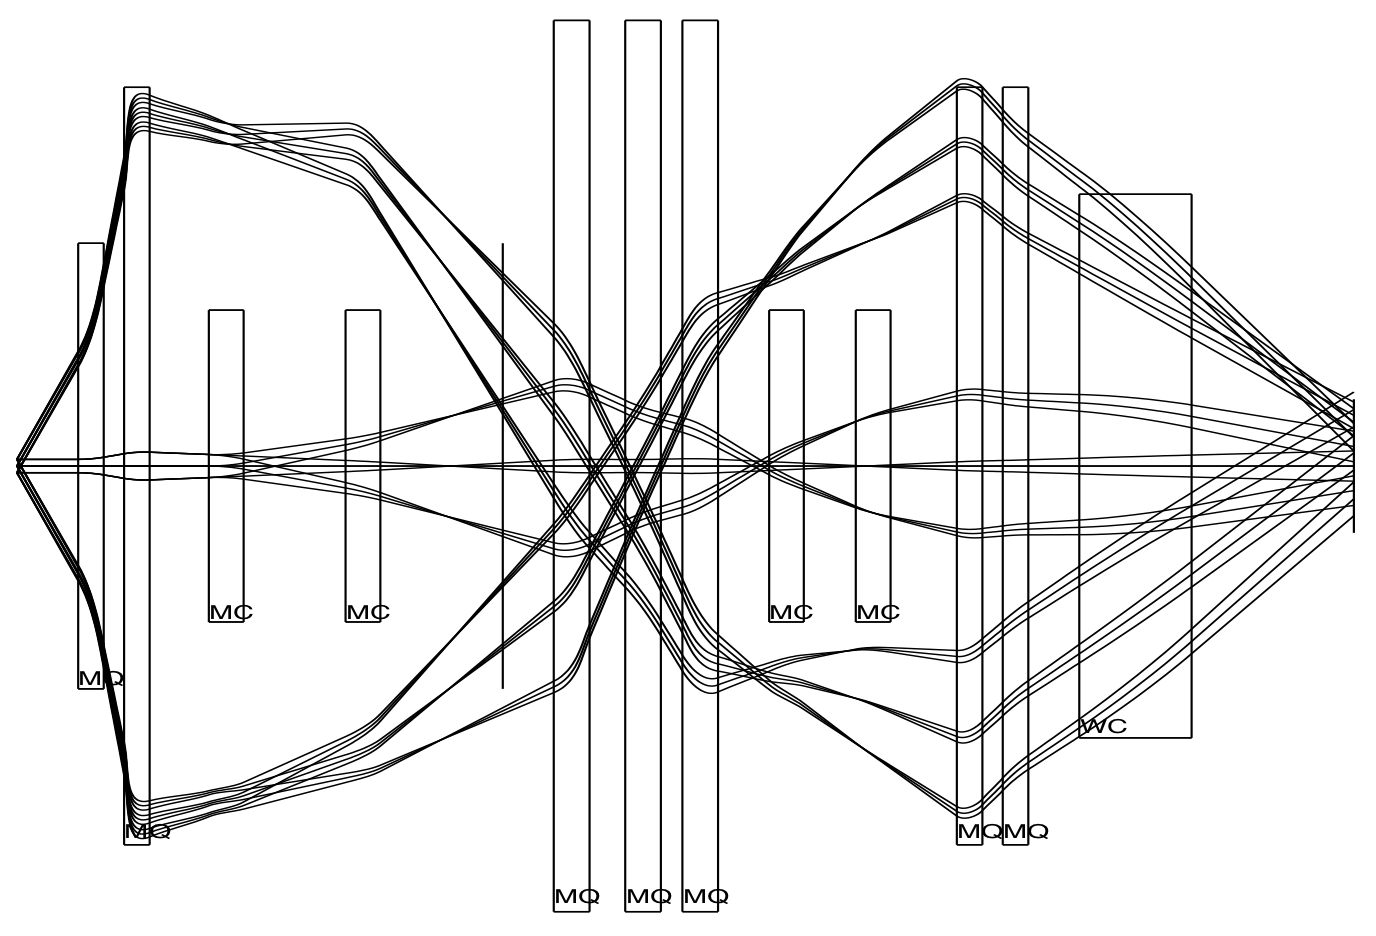
\includegraphics[width=0.8\textwidth]{figures/optimal_tune_x.png} \\
            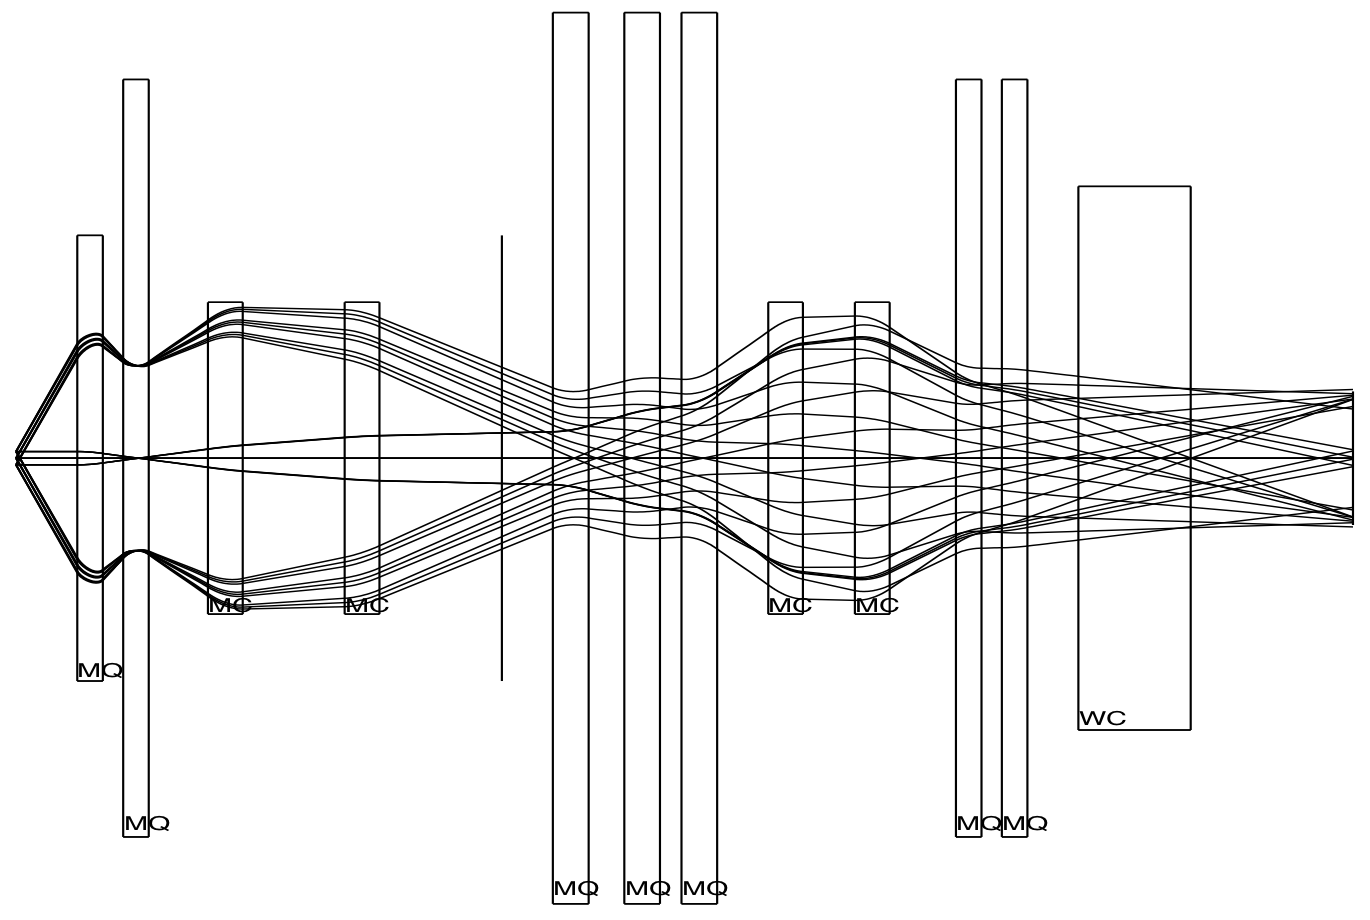
\includegraphics[width=0.8\textwidth]{figures/optimal_tune_y.png}
        }
        \caption[Horizontal and vertical rays through St.\
            George for $\alpha$ particles]{Horizontal (upper plot) and
            vertical (lower plot) rays through St.\ George for the
            altered tune transporting $\alpha$ particles to the
            post-Wien filter focal plane $F_2$. The pole tip fields are
            given in Table~\ref{tab:poletip}.}
    \end{center}
\end{figure}

The initial St.\ George magnetic settings were first found in a similar
manner to the energy and angular acceptance commissioning, with the
primary difference being the initial COSY settings for the magnets.

\subsection{Beam Preparation}

The incident proton beam must be tuned for the desired energy. The beam
energy is set by adjusting the 5U and the analyzing magnet, with the
remainder of the transport beam line adjusted for the new energy. In
situations where the previous energy is close (within a few keV) to the
desired energy, this energy change is relatively straightforward as it
requires smaller changes to the beam line settings.

The incident beam must also be aligned with the magnetic optical axis of
St.\ George in the same manner as described in Sec.~\ref{sec:tuning}.
The magnets at the entrance of St.\ George, namely $Q_1Q_2B_1$ must be
brought down to zero in order to align the incident beam. The collimator
position is also determined in the same manner as the commissioning work
in order to determine the position of the Al target.

Once the beam is aligned, the target is put in place and $Q_1Q_2B_1$ are
recycled and brought to their scaled values for the $\alpha$ particle
energy in question. The recycling procedure ensures that the magnetic
field produced by the magnet is not affected by self-magnetization.

\subsection{Measuring Beam Suppression}

Once the incident beam is prepared, the next step is to see how much of
the beam reaches the detector plane without the target in place. This
step is a direct measurement of the suppression of the separator and is
essential to ensuring that the count rate at the detector due to the
beam is minimal. If the beam current at the detector due to the beam is
too high, it is possible that the detector could be damaged or the
signal of the produced $\alpha$ particles could be lost due to dead time
considerations.

The detector at the focal plane is located behind a thin Al shield when
fully retracted. This shield protects the exposed detector in situations
where the direct beam is incident through St.\ George. To determine if
the residual beam current at the detector plane is too high, the
detector is slowly moved up while the data acquisition system is
running. If the count rate is negligible, the detctor is slowly moved up
in steps until it reaches its final position centered on the magnetic
optical axis.

Using the beam current at the target location, the suppression can be
calculated from the yield of the incident proton beam at the detector
plane. This suppression does not include the target effects, so it can be
considered as an initial estimate of the rejection of the separator. The
rejection is calculated by
\[
    S = \frac{N_{\rm beam at target}}{N_{\rm beam at detector}}.
\]
Initial measurements of the suppression of St.\ George for the altered
tune are approximately $10^{13}$. Once the suppression is determined to
be adequate for the experiment, the detector is again retracted to
behind the shield. The beam at this point is stopped before the target
location to allow for the moving of the detector and target.

\subsection{Target Effects}

The initial beam suppression does not include the effects of the target
on the incident beam. Once the initial suppression has been shown to be
acceptable for the detector, the target is placed into the beam line.
Its position is based on the found collimator position from the initial
beam tuning and alignment.

Once the target is in place, the detector will see $\alpha$ particles
produced in the reaction and any residual beam protons that are
transported to the focal plane. When the beam energy is on resonance,
there is a possibility that the produced $\alpha$ particle count rate is
high enough that there could be damage to the detector when combined
with the potential residual beam. With the detector still behind the
shield, the beam is sent into the target chamber.

As before, the detector is slowly moved up while monitoring the total
count rate at the detector. This count rate will primarily be due to the
produced $\alpha$ particles. Once the detector is fully extended, the
initial production runs to fine tune the settings of St.\ George can be
completed.

\subsection{Final Optimization}

When scaling the elements of St.\ George to the expected $\alpha$
particle energy, both the magnetic elements and the electrostatic plates
of the Wien filter need to be adjusted. The Wien filter voltage is set
according to
\[
    V_{\rm WF} = \frac{d E_{\alpha}}{2 \rho_{\rm WF}},
\]
where $d$ is the distance between the Wien filter plates in meters and
$\rho_{\rm WF}$ is the desired bending radius of the Wien filter. When
the $\alpha$ energy is given in keV, the final voltage will be in kV and
is the set point for each of the two electrodes.

The final Wien filter voltage may differ from this value. The central
energy of the $\alpha$ particles may be slightly different than that
used, the physical electrodes may have slight imperfections which change
the resulting electric field, or the voltage supplied to the
electrostatic plates may be slightly different than the setpoint. For
these reasons, the final tuning of the Wien filter is to center the
$\alpha$ particle count distribution horizontally on the Si detector.
Adjusting the Wien filter voltage to higher (lower) values for a set
magentic field strength will move the $\alpha$ distribution right (left)
in the horizontal plane. An example showing the horizontal
distribution of the $\alpha$ particles is given in
Fig.~\ref{fig:alpha-distribution-strips}.

\begin{figure}
    \begin{center}
        \centerline{
            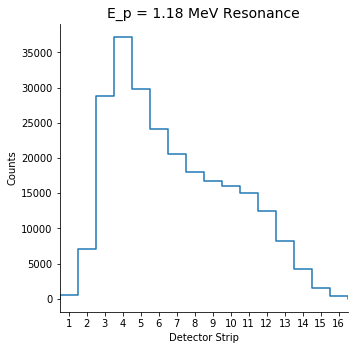
\includegraphics[width=0.4\textwidth]{figures/low_resonance_detector_strips.png}
            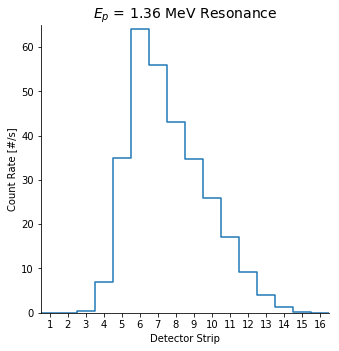
\includegraphics[width=0.4\textwidth]{figures/high_resonance_detector_strips.png}
        }
        \caption[Horizontal $\alpha$ particle distribution]{Horizontal
            $\alpha$ particle distribution at the detector plane after
            the Wien filter settings are optimized. The optimization
            centers the count distribution on the detector by adjusting
            the voltage to swing the beam distribution left or right.
            The runs near each of the resonance peaks are shown. Strip 1
            is on the ``beam right'' side of the detector.}
        \label{fig:alpha-distribution-strips}
    \end{center}
\end{figure}

The $\alpha$ particle distribution potentially extends past the physical
limits of the Si detector in the horizontal and vertical direction.
Centering the distribution horizontally may still miss a small
proportion of counts. For runs that are near the resonance energy, the
counts missed horizontally is a miniscule fraction of the total counts
detected and can be effectively ignored. For runs at energies further
from the resonance energy, the fraction of counts that are missed by the
detector may become a larger fraction of the total counts, requiring
further studies to fully quantify the lost counts. The maximum expected
lost counts is around 1\,\% for our runs furthest from the resonance
energy. Since the acceptance of St.\ George is based on counts reaching
the detector, these lost counts are based on the tune of the separator
and provide an additional metric to measure the capabilities of the
separator.

An additional source of lost counts are those from the $\alpha$
distribution that reach the detector plane above and below the detector.
Due to the limitations of the detector system, only those counts below
the final detector position can be directly measured. As St.\ George is
vertically symmetric, we assume that the count rate above the detector
position is equal to that below the detector system. To measure these
counts below the detector position, the detector is moved down to the
position where the top of the Si detector is at the same vertical
position as the bottom of the detector when it is in its final position.
A figure displaying these positions is shown in
Fig.~\ref{fig:det-position}

\begin{figure}
    \begin{center}
        \centerline{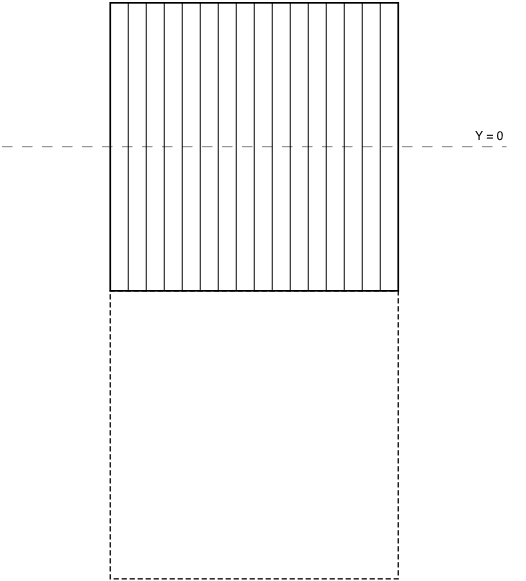
\includegraphics[width=0.8\textwidth]{figures/detector_position.png}}
        \caption[Detector positions]{Detector positions used to measure
            the produced $\alpha$ particles that miss the detector. The
            horizontal missed particles are determined through adjusting
            the Wien filter electrostatic field, since the horizontal
            position of the detector cannot be changed. The individual
            Si strips are vertical, so the actual vertical extent of the
            beam cannot be directly determined. The solid detector is
            the running position, which is centered vertically on the
            beam line. The dashed position is the low detector position
            used to estimate the vertical extent of the beam.}
        \label{fig:det-position}
    \end{center}
\end{figure}

Once these final checks are performed, the detector is returned to its
final position in the center of the beam line. At this point, the actual
measurement of the reaction yield can be measured.

\subsection{Experimental Run}

At each energy, the yield of the produced $\alpha$ particles at the
detector is measured until a given threshold is met. For runs at or near
the resonance energy, data was collected for 15 minutes. The minimum run
time used reduces the possibility that minor fluctuations in the beam
current during the run have an outsized effect on the final yield. For
runs away from the resonance energy, the run was ended once
approximately 20k counts were detected within the expected energy range
of the produced $\alpha$ particles summed across all 16 Si strips. This
minimum count threshold ensures that the statistical uncertainty due to
the counts is less than 1\,\%.

For the final run, the incident beam current and the detector yield are
monitored throughout the run. A beam current measurement is taken before
and after the run to provide an estimate on the beam current during the
entire run. If the run continues for longer than 15 minutes, the current
is also measured every 15 minutes. Due to the design of the target
chamber without an offset Si detector, these periodic beam current
measurements are the only way to infer the changing beam current during
the run that is independent of the counts at the detector. As the beam
is not reacting with the target during these measurements, the time
taken is reduced from the total run time.

Once the run is completed, the beam is stopped and the system\---{}the
5U accelrator, the transport beamline, and St.\ George\---{}are adjusted
for the energy for the next run and the process is repeated.

% Kings County 2.5 yr peated bourbon (Brooklyn, NY)

\chapter{ANALYSIS}
\label{ch:analysis}

The angular acceptance of St.\ George can be determined by comparing the
expected yield from the reaction at the desired energies to the actual
counts measured at the detector plane. If we assume a symmetric angular
acceptance, the opening angle of the acceptance cone can be directly
calculated and compared to the anticipated angular acceptance opening
angle of 40~mrad. The angular acceptance and its uncertainty for each
energy can be determined independently of the other points. The angular
acceptance is based on the properties of the target, incident beam,
detector, and recoil separator and the decisions relating to the
experiment itself.

The measurement of the yields near and on the two resonances can also be used
to determine the properties, such as the resonance strength, related to those
resonances.

% cite python packages here
All code was written using the scientific Python stack (NumPy, SciPy,
MatPlotLib, Pandas, PyMC3). An analysis framework pyne was developed
concurrently in python to aide in direct analysis of the run information
from the raw data files.
% reference appendix ("for more details...")


\section{Target Properties}
\label{sec:target-properties}

% measuring foil thickness should be a sentance or two
% cite stopping power website for SRIM for the SRIM uncertainty (around 3%)
% H and He should be similar
% there is enough data in the energy range in question to justify it

A self-supporting \nuc{27}{Al} target was used for the entirety of the
experiment. The target thickness was measured using an offline detector
station and a mixed \nuc{241}{Am}/\nuc{148}{Gd} alpha-particle source. The
target thickness was measured by observing the energy loss of the two
alpha peaks and using a Monte Carlo method to determine the value and
uncertainty. The measured target thickness is
$63.8^{+2.0}_{-1.7}$~$\mu$g/cm${}^{2}$ (95\,\% confidence interval), which does
not include the uncertainty due to SRIM, and can be used to determine the
energy loss for other particles at any energy.

In our energy range of interest for both protons and $\alpha$ particles, the
uncertainty in the stopping power in the SRIM results is approximately 3-5\,\%,
based on the spread in experimental values from different data sources. To be
conservative, an uncertainty of 5\,\% is adopted for all calculations. When
taking the SRIM uncertainty into account, our measured thickness is
$63.8^{+6.7}_{-6.6}$~$\mu$g/cm${}^{2}$ (95\,\% confidence intervals).

% see foil_thickness/target_thickness_20180403.ipynb

\begin{table}
    \begin{center}
        \caption{ALPHA PARTICLE ENERGIES FOR THE \nuc{241}{Am}/\nuc{148}{Gd}
            MIXED SOURCE}
        \label{tab:mixed-source}
        \begin{tabular}{rS[table-format=2.4]S[table-format=2.4]}
            \toprule
            \midrule
            {\textbf{Isotope}} & {\textbf{Energy [keV]}} &
                {\textbf{Relative Intensity [\%]}} \\
            \midrule
            \nuc{148}{Gd} & 3182.69 & 100   \\
            \nuc{241}{Am} & 5388    &   1.6 \\
                          & 5442.8  &  13.1 \\
                          & 5485.56 &  84.8 \\
            \bottomrule
        \end{tabular}
    \end{center}
\end{table}

% rework below...?
For subsequent calculations, the
thickness used was sampled from this distribution.

The uncertainties present in each step of the procedure laid out above
are automatically propagated forward due to the methods chosen. The
stoichastic nature of the process allows the influence of the base
assumptions of the underlying data (e.g. the counts in each bin are
drawn from a Poisson distribution) to be seemlessly brought forward
without the need of clumbersome mathematics that can potentially hide
wrong assumptions about the values in question, such as that all of the
data is normally distributed.

For most of the following calculations, the number of target nuclei per
square centimeter is used instead of the thickness in $\mu$g/cm${}^{2}$. Our
target thickness is then $1.42^{+0.06}_{-0.06} \times 10^{18}$ nuclei/cm${}^{2}$.
This value is useful for calculating the energy loss of the proton
through the target, as that relies on the number density of the target
and the stopping power of the material. The energy loss of the beam will
be discussed in the next section.


\section{Beam Properties}
\label{sec:beam-properties}

The incident proton beam was produced by the 5U and delivered to the St.
George target area. The beam energy and resolution were determined
through a series of accelerator and beamline commissioning experiments
performed before this experiment was performed.

% Similar experiments showed that the energy resolution
% of the beam is approximately 300 keV. To be conservative, a value of 500 keV
% was used for all runs.

The beam energy was determined from the calibration of the 5U analyzing
magnet performed during a different experiment. During the experiment,
the magentic changes were performed slowly such that the magnetic field
did not appreciably drift during the runs. The energy resolution can
also be determined from the calibration runs, where the resolution is
given by the energy width of the leading edge of the resonance scan.
Values of approximately 300 eV were commonly observed, with a
conservative value of 500 eV adopted for this experiment since no direct
energy calibration was performed with our specific experimental setup.
The uncertainty in the analyzing magnet field is accounted for within
this uncertainty and is not considered separately.

% While the uncertainty in the field strength recorded is
% not completely negligible, it is included within the beam energy resolution
% and is not considered separately.

The beam current was relatively stable during the experiment. During the
longer runs, the beam current was measured every 15 minutes in order to
monitor its change during the run. For each run, the current uncertainty
was determined by the measured values for cases where multiple current
measurements were performed, or 5\,\%. For all runs, the final current
uncertainty was between 5 and 12\,\%. Ideally, an offset Si detector at
the target location would be used to monitor the beam current during the
entirety of the run by measuring the current of the scattered beam
particles at a fixed angle. As this setup was not available for the
target chamber, periodic direct measurements of the current using the
Faraday cup at the target location were required to measure the beam
intensity.

\section{Detector Properties}
\label{sec:detector-properties}

A 16-strip Si detector was used to detect the produced alpha particles
during the experiment. A calibration run was performed following the
experiment using the same detector and data acquisition settings as used
during the experiment. A \nuc{241}{Am}/\nuc{148}{Gd} mixed alpha source was used
for calibrating the energy conversion and energy resolution of each
strip separately. All of the strips were similar with approximately 2
keV/bin for the calibration and approximately 2.75\,\% (90~keV) for the
energy resolution.

The calibration run resulted in a single spectrum. Due to the poor
energy resolution of the detector resulting from the lower-than-optimal
bias voltage setting used during the experiment, only the two highest
intensity peaks could be resolved above the background. As the alpha
peak resulting from \nuc{148}{Gd} is closer in energy to the alpha
particles produced in the experiment, The alpha peaks also exhibit long
low-energy tails such that the particles produced in the reaction are
smeared out in energy. For the experimental run, an energy threshold was
set to exclude incident proton counts, where counts appearing above the
threshold are considered to be from alpha particles. That threshold was
set by the following:

\begin{equation}
    E_{\rm proton} + 3 \sigma_{\rm beam} + 3 \sigma_{\rm resolution}
\end{equation}

The detector efficiency was not directly measured and assumed to be
100\,\%. Efficiency measurements performed during the commissioning work
supporting the St.\ George detector system resulted in efficiencies above
99\,\% for all strips.

A simulation of the expected energy spectrum at the target location was
performed using SRIM data tables. The simulation looked at the known
energy loss within the target of the incident beam, the expected cross
section within the energy limits of the target, the energy loss of the
produced alpha particles through the remainder of the target, and the
energy resolution of the detector to generate an expected energy
spectrum. The procedure for this simulation is as follows:


\textbf{Step 1:}
  An energy deviation drawn from the Normal(0, sigma) distribution
  (where sigma is the beam energy resolution) for 2000 particles. This
  energy deviation is the difference in energy from the central energy.

\textbf{Step 2:}
  SRIM files for the central energy were generated for fractional depths
  within the target, where the output is the beam energy profile at that
  target depth.

\textbf{Step 3:}
  Using the expected cross section from the AZURE2 R-matrix calculation,
  a depth for each of the simulated particles was generated to determine
  the location within the target that the reaction takes place.

\textbf{Step 4:}
  A beam energy $E_d$ is generated from the distribution of beam energies
  at the given depth, and the initial deviation for that particle is
  added to the energy to give the final beam energy.

\textbf{Step 5:}
  The beam energy is converted to the produced alpha particle energy
  through the kinematic equation

% for some reason, using mnuc didn't work...?
\begin{equation}
    E_{\alpha} = Q + E_{\rm p}\left(
        1 - \frac{m_{\rm p}}{m_{\rm p} + m_{{}^{27}\rm{Al}}} %m_{\mnuc{27}{Al}}}
    \right)
\end{equation}


\textbf{Step 6:}
  The deviation of the alpha particle from a known alpha energy (used to
  generate SRIM files at various depths) was recorded.

\textbf{Step 7:}
  An alpha energy was generated for each particle based on the remainder
  of the target that it needs to travel through from the final energy
  distribution generated for particles traveling through that thickness.

\textbf{Step 8:}
  The energy deviation is added back to the alpha particle's energy to
  give its final energy.

This procedure generates an alpha-particle energy spectrum following the
target location given the known parameters about the target thickness
and the cross section, and incorporates the known energy resolution of
the incident alpha beam and the stoichastic nature of the energy loss
and reaction within the target. Finally, using the known energy
resolution of the detector, a final energy spectrum can be generated by
drawing new alpha particle energies from the distribution:

\begin{equation}
    E_{\alpha,\rm{detector}} \sim \rm{Normal}(E_{\alpha},\sigma_{\rm detector})
\end{equation}

An example of the output of this procedure is given in {[}FIGURE{]},
where the agreement between the location and width of the alpha peak can
be seen in the normalized spectra. Note that the low energy tailing of
the detected particles is not modeled in our simulated spectrum, as we
don't know the full characteristics for the detector response.


\section{Additional Parameters}
\label{sec:additional-parameters}

Additional inputs into the final calculation of the acceptance of St.
George are the cross section determined from an R-matrix fit on several
low-lying resonances, the stopping power of protons in aluminium from
SRIM, the run time, and the counts at the detector. For those parameters
that are derived from external programs (AZURE2 and SRIM), the
uncertainty is assumed to be negligible. The uncertainty in the time was
assumed to be 10 seconds for those runs that only lasted for a single
15-minute span, and higher for those runs that required the periodic
measurement of the beam current which resulted in stopping the incident
beam for an unspecified duration of time.

The counts at each detector were the sum of all events above the
threshold defined by the beam energy and detector resolution. The counts
are Poisson distributed, with the length of time for the run was such
that the uncertainty from the counts at the detector was not above 5\,\%,
with most runs having a count uncertainty of a much lower value. The
direct uncertainty of the counts at the detector is partially convolved
with the run time; a lower counting uncertainty requires a longer run
time and potentially a larger time uncertainty.

The direct beam reduction by St.\ George must be on the order of
$10^{10}-10^{14}$ in order to avoid damaging the Si detector and to
measure lower value regions of the cross section. This requirement is
within the designed capabilities of St.\ George when tuned for heavy
recoil transmission to the final detector plane, but must be verified
experimentally due to the altered tune and different detector plane
required for this experiment. During the experiment, count rates at the
detector were monitored, and potential counts from the direct proton
beam were excluded from the final counts with the energy discriminator
previously described.

\section{Final Acceptance Measurements}
\label{sec:final-acceptance-measurements}

The acceptance of St.\ George can be found for each energy value by
comparing the detected counts to the expected yield for that incident
beam energy. The yield is found from:

\begin{equation}
    Y(E) = \frac{N_r}{N_b},
\end{equation}

where $N_r$ is the number of reaction products produced and $N_b$ is the
number of incident beam particles. We can determine $N_b$ from the beam
current and the total run time. The value for $N_r$ is determined by the
total counts at the detector (for the experimental yield) or the
integration of target and cross section properties following

\begin{equation}
    Y(E_0) = \int \frac{\sigma(E)}{\epsilon(E)}\,\rm{d}E
\end{equation}

In both cases, the detector efficiency and St.\ George transport
efficiency are 100\,\%, as previously discussed.

The acceptance in mrad is given by

\begin{equation}
    \theta = \arccos\left(1 - 2 \frac{Y_{\rm experiment}}{Y_{\rm theory}}\right)
\end{equation}

The angular acceptance can be calculated in this way for each run
individually, as shown in FIGURE and TABLE. The process for
calculating the uncertainty bounds is given by the following, repeated
2000 times to have enough confidence in the final values:

\textbf{Step 1:}
  The beam energy, beam current, and time are sampled from a normal
  distribution $\rm{Normal}(\mu,\sigma)$, where $\mu$ and $\sigma$ are for the value
  (energy, current, or time) in question.

\textbf{Step 2:}
  The incident number of particles is calculated from the current and
  time.

\textbf{Step 3:}
  The target thickness in energy is calculated from finding the stopping
  power at the incident beam energy from the SRIM tables, and sampling
  from the distribution of target thicknesses in terms of atoms/cm${}^{2}$.

\textbf{Step 4:}
  The yield is determined by integrating EQUATION between the
  entrance energy and the lower energy given by that entrance energy
  minus the target thickness.

\textbf{Step 5:}
  The experimental yield is drawn from a poisson distribution
  $\rm{Poisson}(c)$, where $c$ is the number of counts detected.

\textbf{Step 6:}
  The acceptance for the iteration is caluclated by EQUATION.

The distribution of values generated by the process above can be used to
find the acceptance and confidence intervals for the run in question.
Each run has an acceptance described by its distribution, which is the
run for that particular setting of St.\ George.


\section{Resonance Parameters}

Determine resonance parameters

Find area under yield curve

Relate to equation

Repeat a bunch of times to include energy, yield, and acceptance uncertainty (?)

Two to find: resonance strengths, reaction rates

\chapter{DISCUSSION AND CONCLUSION}
\label{ch:discussion-and-conclusion}

The experiment was designed to experimentally confirm an aspect of the
acceptance for St.\ George, specifically the angular acceptance at small
energy deviations, using a well-known reaction. Additionally, the
experiment aimed to allow for an additional set of reactions to be
studied using the facility. The technical capabilities of the separator
system were shown to be adequate even with sub-optimal characteristics
in the experimental setup, opening up the possibilities of studying low
energy $(\rm{p},\alpha)$ reactions in the future. The angular acceptance at the
peak of the resonances was shown to be consistent with the desired design
characteristics of the separator.


\section{Advantages and Disadvantages}
% from call with Manoel: 2018-05-16
(p,a) can suffer from elastic scattering, but St. George can avoid that by
looking at zero degrees. Ratio of alphas to elastically scattered protons
can have a prohibitivve count rate

Disadvantage: no angular distribution, requires recoil separator
Advantage: can avoid killing detectors, check zero degree


\section{Uncertainties}
\label{sec:uncertainties}

%% NOTES

systematic: alphas hitting interior walls, energy cutoff at detector,
transmission (faraday cup offset?)

Missed counts can be measured, say that target cup roughly restricts to 40 mrad
in all directions, so those additional counts could be from within 40 mrad (I
feel weird about this, so don't directly add it in, but mention the amounts
either here or in potential sources of error)

%% END NOTES

The final uncertainties on the acceptances at each run energy are skewed
distributions. Since basic error propagation relies on the errors being
gaussian distributed, the fact that our uncertainties are not partially
justifies the Bayesian approach described previously. Part of the reason
for the skewed distributions is that the acceptance is bounded by zero
and $\pi/2$, and since our distributions sit closer to the zero end instead
of near the middle of the range somewhat requires that the distribution
be skewed.

\subsection{Statistical}

The uncertainties on most of the inputs are gaussian distributed, as
that represents the statistical nature of the process that creates that
input value. For example, the beam current in gaussian distributed
because...

DISCUSS

The final uncertainty bands for each of the acceptance measurements can
be analyzed by what values affect the range for the uncertainty. We can
limit this discussion to inputs that are controllable by the
experimenter. The final uncertainty will be made up of the uncertainty
from inputs and the uncertainty from those statistical and irreducible
processes. The four inputs that the experimenter can control are the
energy, time, current, and thickness uncertainties. The energy
uncertainty is related to the stability of the accelerator and the
calibration of the analyzing magnet, both of which can be measured and
regulated to the point where the uncertainty can be minimized. The time
uncertainty is based on the total runtime and the interruptions caused
by requiring the stoppage of the beam in order to measure the current
and can be reduced through synchronization of the DAQ with the start of
bombardment, and by minimizing interruptions during the data collection
process. The current uncertainty can be minimized by measuring the
current continuously during the experiment, as there will then be fewer
unknown changes in the beam current and a single value for the beam
current does not need to be applied to the entirety of the experimental
run. Finally, the thickness uncertainty can be minimized by performing
target thickness measurements at multiple energies and with potentially
multiple particles, and by running those measurements for longer such
that the energy loss by the particles can be more accurately determined.

Each of these inputs affects a different part of the final acceptance,
based on how it relates to the experimental and theoretical yield, or
both. We can determine the impact of reducing the uncertainty on each of
these inputs by setting the uncertainty to zero within the analysis
pipeline, which would return a different uncertainty band for the run in
question. Since these uncertainties are not necessarily independent of
each other, we should also look at all combinations of these four inputs
being controlled for to get a full picture of the impartances.
Additionally, the irreducible uncertainty can be determined by keeping
all of the inputs constant. The contribution to the final uncertainty is
expressed as a percent of the total uncertainty band for both the 67\%
and 95\% confidence interval, so the amount of the band that is
accounted for by the inputs that are not held constant.

TABLE_67
TABLE_95

From these tables, we observe a few interesting trends that we can
leverage during follow-up experiments to improve the final uncertainty
of the acceptance and from that the uncertainty on the experimental
yield. The trends are...

DISCUSS

\subsection{Systematic}


\section{Uniformity of Acceptances}
\label{sec:uniformity-of-acceptances}

When calculating the acceptance for St.\ George, it was assumed that the
acceptance cone was described by a single opening angle. In practice,
the horizontal and vertical opening angles may be distinct from each
other. During preliminary experiments for the acceptance of St.\ George,
it required much less fine tuning of magnetic fields to achieve the
maximum vertical acceptance than it was to achieve the maximum
horizontal acceptance. This observation may be due to the lack of
dispersive elements in the vertical plane.

The strips of the Si detector were aligned such that an individual strip
was oriented in the vertical direction, or a particle that is deflected
horizontally would be detected on a different strip (see FIGURE).
This orientation allowed for improved tuning in the horizontal plane
with the lack of sensitivity in the vertical plane. The auxiliary runs
performed where the detector was place in the ``low'' position (where
the top of the detector is located where the bottom of the detector
would be in the regular running position) inform the amount of particles
that are not captured in the vertical plane due to minor mistuning of
the separator, and the auxiliary runs used to center the produced alpha
particle distribution on the detector horizontally inform the amount of
particles that are not captured in the horizontal direction. Ideally, a
detector segmented in both the horizontal and vertical plane would give
a full description of the alpha-particle beam spot density at the
detector plane and could be used to better relate the distribution of
counts at the detector plane to the acceptance cone at the target
location.

In the final configuration of the target system, a series of conical
collimators will be located following the target location to defined the
40 mrad acceptance cone. As the desired configuration of St.\ George is
to measure $(\alpha,\gamma)$ reactions where the heavy recoil particles are
emitted from the target within a cone with an opening angle less than 40~mrad,
NOTES. For experiments similar to this where the ejected
particles are emitted within a cone larger than 40~mrad, these
collimators would ensure that the particles reaching the final detector
must have been emitted within that known acceptance cone. This
restriction would improve the tuning of the separator for similar
experiments, as the emitted particle beam spot at the detector plane can
be more easily tuned to fit completely on the detector.


\section{Potential Sources of Error}
\label{sec:potential-sources-of-error}

The preliminary tunes were determined by keeping a beam with a given
energy and angular deviation from the mean reached the detector plane
within the physical space of the detector as measured on a quartz.


\section{The $(\rm{p},\alpha_1)$ channel}
\label{sec:the-palpha_1-channel}

At the resonances probed, the $(\rm{p},\alpha_1)$ reaction channel is also
open. Measuring the cross section for this reaction at the two desired
resonances is a more difficult experiment due to the lower rigidity of
the produced alpha particles due to the lower energy. The kinematics for
this reaction are given in TABLE.

The lower rigidity is still within the design parameters of St.\ George,
but due to the altered tune required to direct the produced alpha
particles to the detector plane has different rejection properties than
the standard tune. As such, the incident proton beam is close enough in
rigidity that the beam may strike the detector. The beam reduction
levels would not be high enough to avoid damaging the Si detector,
preventing the measurement of the cross section without either
additional rejection capabilities or an improvement in the tune.

MORE DETAILS FROM LOGBOOK


\section{Requirements for Replication and Improvement}
\label{sec:requirements-for-replication-and-improvement}


\section{Next Steps}
\label{sec:next-steps}


\section{Closing Thoughts}
\label{sec:closing-thoughts}


\appendix
\chapter{RUN INFORMATION}

Additional information about the \alpa{} productions runs.

\begin{table}
    \begin{center}
        \caption{RUN ENERGY DETAILS}
        \label{tab:run_energy}
        \begin{tabular}{cS[table-format=5.2]S[table-format=2.6]%
                S[table-format=2.6]}
            \toprule
            \midrule
            \textbf{Run Numbers} & \textbf{Field [G]} & \textbf{$E_p$ [MeV]} &
                \textbf{$E_{\alpha}$ [MeV]} \\
            \midrule
            261\----{}264          & 1693.3 & 1.36318 & 2.7700 \\
            265\----{}270$^\dagger$ & 1690.4 & 1.35852 & 2.7655 \\
            271\----{}277          & 1687.1 & 1.35322 & 2.7604 \\
            278\----{}282          & 1683.9 & 1.34809 & 2.7554 \\
            283\----{}288          & 1680.1 & 1.34201 & 2.7495 \\
            242\----{}248          & 1580.8 & 1.18807 & 2.5996 \\
            251\----{}255          & 1577.5 & 1.18311 & 2.5948 \\
            256\----{}260$^\dagger$ & 1574.6 & 1.17876 & 2.5905 \\
            229\----{}234          & 1571.4 & 1.17398 & 2.5859 \\
            235\----{}241          & 1567.9 & 1.16875 & 2.5808 \\
            \bottomrule
        \end{tabular}
        
        \vspace{0.5em}
        $\dagger$: Denotes runs at resonance energy
    \end{center}
\end{table}

\chapter{DEFLECTOR SETTINGS}

Deflector settings used for commissioning work. Voltages are based on
the physical characteristics of the deflector system and the beam
properties to provide the necessary deflection. Setpoints are based on
the version of the control program in place at the time of the
experiments.

\begin{table}
    \begin{center}
        \caption{DEFLECTOR SETTINGS FOR TEST BEAMS}
        \label{tab:deflector}
        \begin{tabular}{S[table-format=2.0]S[table-format=2.4]%
                S[table-format=2.0]S[table-format=2.4]S[table-format=3.0]}
            \toprule
            \midrule
            & \multicolumn{2}{c}{\textbf{$\mnuc{1}{H}^{+}$ at 1 MeV}} &
                \multicolumn{2}{c}{\textbf{$\mnuc{4}{He}^{+}$ at 2.3
                MeV}} \\
            {\textbf{Angle [mrad]}} & {\textbf{Voltage [kV]}} &
                {\textbf{Setpoint}} & {\textbf{Voltage [kV]}} &
                {\textbf{Setpoint}} \\
            \midrule
            5  & 0.363 &  9 & 0.834 &  24 \\
            10 & 0.725 & 20 & 1.668 &  49 \\
            15 & 1.087 & 31 & 2.501 &  74 \\
            20 & 1.450 & 42 & 3.335 & 100 \\
            25 & 1.813 & 53 & 4.170 & 125 \\
            30 & 2.176 & 64 & 5.004 & 150 \\
            35 & 2.539 & 75 & 5.839 & 175 \\
            40 & 2.902 & 86 & 6.674 & 201 \\
            45 & 3.265 & 97 & 7.509 & 226 \\
            \bottomrule
        \end{tabular}
    \end{center}
\end{table}

\chapter{ANALYSIS PACKAGE}
\label{ch:pyne}

The analysis and plots contained within this dissertation were completed
using Python and a small set of standard scientific python packages:


\begin{description}
    \item[Matplotlib] a 2D plotting package that supports multiple
        backends and output formats
    \item[NumPy] a standard numeric package for array (vector and
        matrix) computing
    \item[Pandas] a tabular data interface that organizes heterogeneous
        data into simple to use and manipulate data structures
    \item[PyMC3] a probabilistic programming language in python useful
        for Bayesian inference
    \item[SciPy] a scientific utilities package built on top of NumPy
        that includes general-purpose routines such as curve fitting,
        root finding, signal processing and more
\end{description}

These packages are standard components of the Python Scientific Stack,
and their usage and internals are well-documented and trusted by many
scientists in multiple fields. The usage of Python in the scientific
community has increased steadily over the years, with multiple special
purpose packages built on top of the foundation of these three packages,
particularly NumPy.

For the actual analysis, a two-part analysis framework was developed in
tandem with the analysis work: Python for Nuclear Experiments (PyNE) and
the St. George Analysis Package (SAP). These packages are designed to be
extensible by other research groups, guided by the requirements of the
St. George group, while providing an easy-to-use and understand
object-oriented interface to performing nuclear astrophysics research.
Development work was chronicled on the packages' GitHub
page\footnote{\url{https://github.com/mmoran0032/pyne}}, and may be
installed from there.

These packages would not be possible without two other important
packages: the ROOT\footnote{\url{http://root.cern.ch/}} Data Analysis
Framework\cite{ROOT} and
\texttt{evt2root}\footnote{\url{https://github.com/ksmith0/evt2root}}.


\section{Python for Nuclear Experiments}

The PyNE package provides base functionality for interacting with
experimental data generated through the standard data acquisition
systems in use at the Nuclear Science Laboratory at the University of
Notre Dame. The package was designed to provide a base pythonic
interface to the data files, including converting them into data files
that work easily with standard python scientific packages. The
underlying purpose for PyNE is not to be an end-to-end analysis package,
but provide the necessary structure to such an end-to-end analysis
package with a common and simple API.

The primary functionality is the organizing of experimental data. From
binary files in either (currently) \verb+.Chn+ or \verb+.evt+ format,
the data is converted into \verb+numpy.ndarray+ format. A logical
directory structure is set up, with run metadata extracted from the
binary files stored in a local JSON file.

Within the API, the data can be easily queried and worked with. The
provided \verb+pyne.Data+ objects (subclassed for channel and event
data) implement the iterator protocol over the ADCs. In this way,
concise and clear analysis on the entire 16-strip detector can be
accomplished through code as simple as the following:

\begin{python}
import pyne
from local_analysis import determine_counts

data_obj = pyne.EVTData('data/run0808')
data_obj.load_data()

total_counts = sum(
    determine_counts(d) for d in data_obj.adc
)
\end{python}

By creating objects that encapsulate the data and meta-data, the
end-to-end analysis becomes much easier, as details about a run and
exploratory work are vastly simplified.

\section{St. George Analysis Package}

For most analysis, there is a need for more work than just finding the
total number of counts. For the experiment conducted within this
dissertation, a few routines were standardized within an add-on package
to PyNE called SAP. Since PyNE just provides the primitive
classes for analysis, any number of extension packages may be produced
building upon that core functionality.


\section{Justification}

Python has become a leading programming language across a range of uses
and industry, led primarily by its data analysis, data science, and
machine learning applications\footnote{Why is Python Growing So Quickly?
\url{https://stackoverflow.blog/2017/09/14/python-growing-quickly/}}.
The three main data analysis packages for python\---{}numpy, pandas, and
matplotlib\---{}have become essential tools in a variety of cases,
especially within the sciences. Packages built upon this base, such as
SunPy\footnote{\url{https://github.com/sunpy/sunpy}} (Python for Solar
Physics), AstroPy\footnote{\url{https://github.com/astropy/astropy}},
Biopython\footnote{\url{https://github.com/biopython/biopython}}, and
many others have been written, tested, and used by researchers all
around the globe. Ground-breaking scientific discoveries, such as the
detection of gravitational waves by LIGO, have been made using Python
as one of the primary analysis
languages\footnote{\url{https://losc.ligo.org/s/events/GW150914/GW150914_tutorial.html}}.
Python has become a \emph{de facto} language for data analysis in many
circles (outside of statistics where
R\footnote{https://www.r-project.org/} is still the primary language),
an adopting it for nuclear astrophysics should not be far behind.

There is a current package
\verb+becquerel+\footnote{\url{https://github.com/lbl-anp/becquerel}}
that has been under development since October 2016 by users at LBNL. As
this package was not known about at the start of my analysis, it was not
used, but it could be possible to use it as a replacement for SAP with
a transformation layer between PyNE and the routines within Becquerel.
There are some very interesting examples of using Becquerel for nuclear
physics analysis that can be viewed in the examples folder in the GitHub
repo. If I were completing this analysis now, I would have stopped at
the data translation layer in PyNE and moved into writing routines that
use Becquerel for the heavy analysis work.

For those thinking that the ``slow'' speed of python will hold them back
from performing large-scale analysis, or that python might not fit with
the use cases that the researcher has, I emplore you to watch Jake
VanderPlas's
keynote\footnote{https://www.youtube.com/watch?v=ZyjCqQEUa8o} from PyCon
2017. One additional point is that the speed of execution is most likely
not the limiting factor in the analysis, but the speed of the researcher
to write, debug, and understand the code may very well be that
bottleneck. Additionally, the use of Jupyter
Notebooks\footnote{\url{https://jupyter.org/}} for code alongside
documentation allows for a lower barrier to entry for rerunning and
understanding experimental analyses years later.

As a user of python since 2007, I have seen large changes in the python
ecosystem and have gradually included python more and more into my own
work. Right now, I owe my career to python and the open source data
analysis packages, and I don't expect that fact to change any time soon.
While my work has shifted from curve fitting to gradient boosted trees
and neural networks, it is still in python, and in many cases the final
understanding of my complex models comes down to dot products in
\verb+numpy+ and plotting with \verb+matplotlib+.

This dissertation would not have been possible without the countless
hours of work and throusands of open source contributions to these core
data analysis libraries and python itself.


% Bibliography and index
\backmatter

\bibliographystyle{nddiss2e}
\bibliography{references}

\end{document}
\endinput
